\chapter{Experimentální výsledky} \label{chapt:experiments}
Tato kapitola prezentuje výsledky experimentů popsaných v sekci~\ref{sec:experiments-design}. 
Cílem těchto experimentů je zhodnotit výkonnost jednotlivých kvantově inspirovaných evolučních algoritmů a provést jejich porovnání s klasickými evolučními algoritmy. 

Nejprve jsou uvedeny výsledky ladění parametrů pro jednotlivé kvantově inspirované evoluční algoritmy. 
Tyto optimalizované parametry jsou následně aplikovány na rozsáhlejší instance problému batohu, jejichž výsledky jsou rovněž prezentovány. 
Každý ze zobrazených grafů je navíc doplněn o informaci z tabulky~\ref{tab:experiments-design}, která uvádí optimální hodnotu řešení problému batohu pro jednotlivé velikosti testovaných instancí.

Na základě získaných dat je v závěru kapitoly vedena diskuze porovnávající klasické evoluční algoritmy s běžnými optimalizačními metodami, a to včetně analýzy jejich silných a slabých stránek. 
Zvláštní pozornost je věnována rovněž vzájemnému srovnání jednotlivých kvantově inspirovaných evolučních algoritmů. 

Ve všech grafech prezentujících výsledky experimentů je použito označení ve formátu (\texttt{alg}-\texttt{inst}), kde \texttt{alg} označuje použitý algoritmus a \texttt{inst} velikost instance problému. 

\section{Kvantově inspirovaný genetický algoritmus}\label{sec:exp-qiga}
V této části jsou představeny experimentální výsledky týkající se kvantově inspirovaného genetického algoritmu (\emph{QIGA}). 
Pozornost je věnována zejména vlivu různých hodnot parametru úhlu rotace $\Delta\theta$ a velikosti populace na kvalitu nalezených řešení. 

\begin{figure}[ht!]
    \centering
    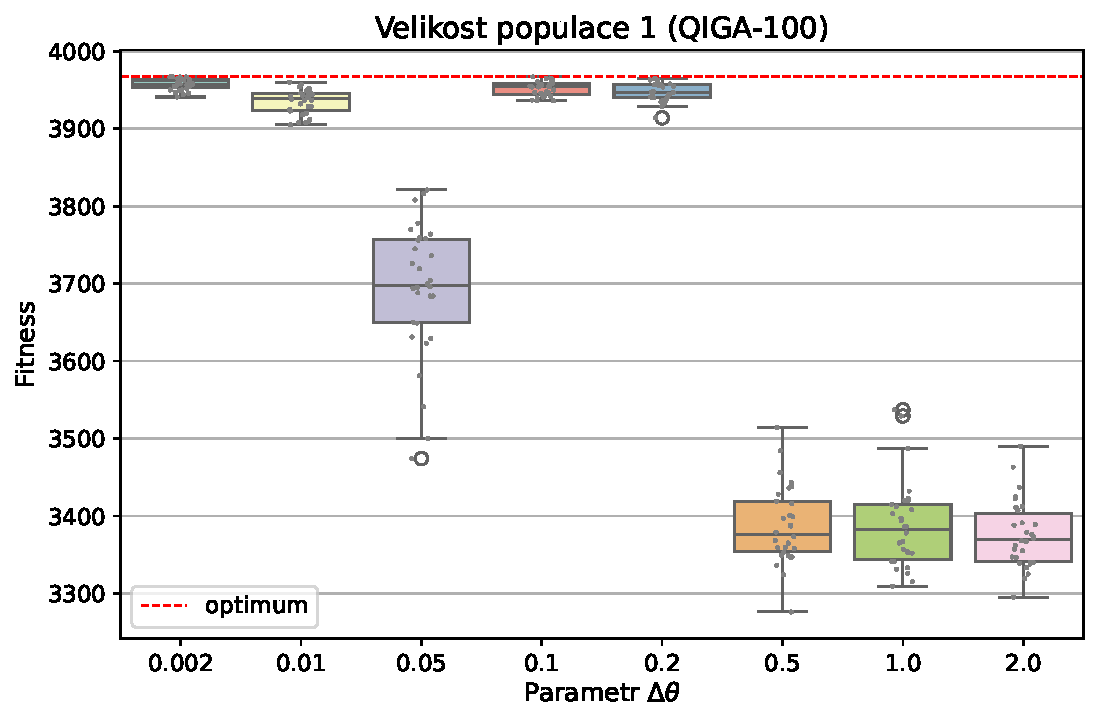
\includegraphics[width=0.7\textwidth]{qiga/boxplot_qiga_100_popsize_1.pdf}
    \caption{Vliv hodnot parametru $\Delta\theta$ při velikosti populace 1. Data prezentovaná na grafu byla získána algoritmem \emph{QIGA} na instanci velikosti 100 pomocí 30 nezávislých běhů s 10\,000 evaluacemi na běh pro každou kombinaci prezentovaných parametrů.}
    \label{fig:qiga-pop1}
\end{figure}

Na obrázku~\ref{fig:qiga-pop1} jsou zobrazeny výsledky experimentů pro problém o 100 položkách s~populací tvořenou jediným jedincem.
Sledován je vliv různých hodnot parametru $\Delta\theta$, jejichž konkrétní nastavení vychází z tabulky~\ref{tab:qiga-all-instance}. 
Prezentovány jsou pouze výsledky pro jednoho jedince, neboť algoritmus \emph{QIGA}, jak bylo uvedeno v sekci~\ref{sec:experiments-design}, neobsahuje mechanismus pro sdílení informací mezi jedinci v populaci. 

Z dat na obrázku~\ref{fig:qiga-pop1} vyplývá, že parametr $\Delta\theta$ má významný vliv na kvalitu řešení. 
Nejlepších řešení bylo dosaženo při $\Delta\theta = 0{,}002$, kde se průměrná kvalita řešení pohybovala velmi blízko optimu a současně vykazovala nejnižší rozptyl. 

Obecně platí, že nižší hodnoty parametru $\Delta\theta$ vedly k lepším výsledkům s výjimkou anomálie při $\Delta\theta = 0{,}05$. 
Naopak vyšší hodnoty (zejména od $0{,}5$ a výše) vedly ke znatelnému zhoršení kvality řešení, doprovázené vyšší směrodatnou odchylkou, což naznačuje nižší stabilitu algoritmu. 
Z výsledků lze usuzovat, že vyšší hodnoty $\Delta\theta$ způsobují velkou změnu kvantového stavu, což má za následek spíše chaotické a méně efektivní prohledávaní prostoru možných řešení. 

Na základě předchozích výsledků byly z dalších experimentů vyřazeny hodnoty parametru $\Delta\theta = 0{,}5, 1$ a $2$, neboť opakovaně vedly k výrazně horším výsledkům. 
Hodnota $\Delta\theta = 0{,}05$ však byla ponechána, ačkoliv také nepatřila mezi nejúspěšnější, neboť spadá do oblasti hodnot, které v jiných případech vedly k velmi kvalitním řešením. 
Právě z tohoto důvodu byla tato anomálie zachována i v následujících experimentech, aby mohla být dále analyzována ve vztahu k větším instancím problému. 

Tato anomálie byla dále zkoumána v kontextu různých velikostí populace, respektive v~závislosti na celkovém počtu vyhodnocení fitness funkce. 
Výsledky zobrazené na obrázku~\ref{fig:qiga-100-all} ukazují, že vliv velikosti populace na kvalitu řešení při nastavení parametru $\Delta\theta = 0{,}05$ není přímočarý. 
Nejhorší výsledky byly dosaženy při populaci tvoření jediným jedincem. 
Se zvyšujícím se počtem jedinců se však kvalita zlepšovala a nejlepších výsledků bylo dosaženo při desítkách jedinců v populaci. 
Při dalším zvyšování velikosti populace však kvalita opět začala mírně klesat.

\begin{figure}[ht!]
    \centering
    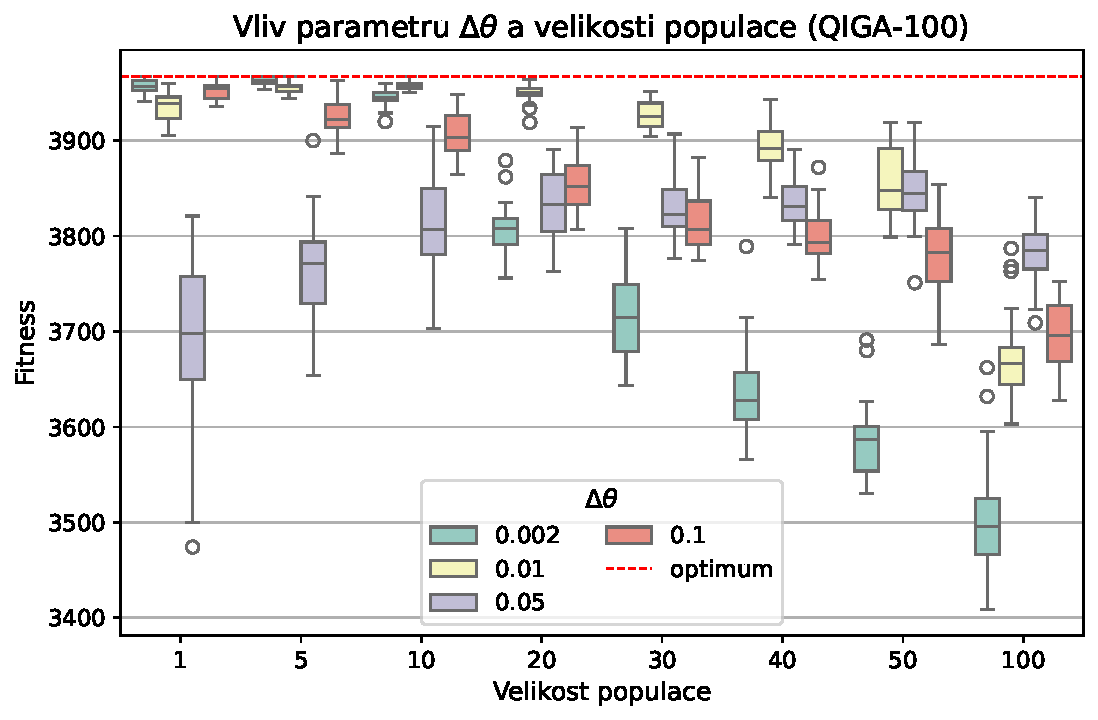
\includegraphics[width=0.87\textwidth]{qiga/boxplot_qiga_100_all_theta.pdf}
    \caption{Závislost kvality řešení na velikosti populace pro různé hodnoty parametru $\Delta\theta$. Data prezentovaná na grafu byla získána algoritmem \emph{QIGA} na instanci velikosti 100 pomocí 30 nezávislých běhů s 10\,000 evaluacemi na běh pro každou kombinaci prezentovaných parametrů.}
    \label{fig:qiga-100-all}
\end{figure}

\begin{figure}[ht!]
    \centering
    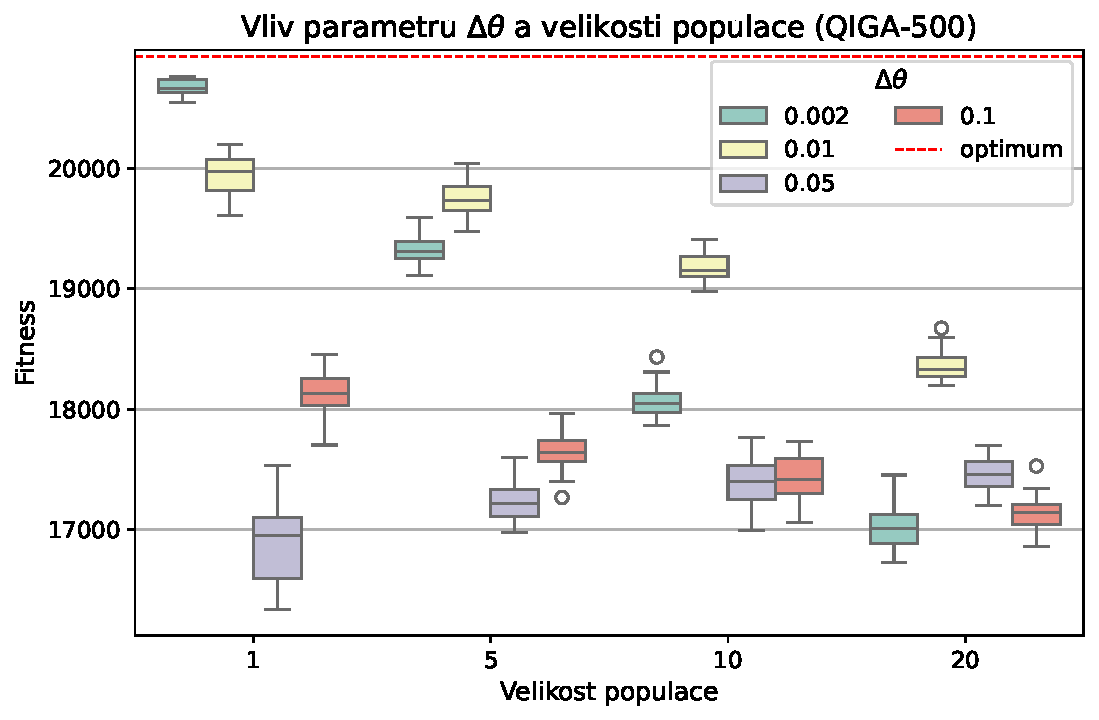
\includegraphics[width=0.87\textwidth]{qiga/boxplot_qiga_500_all_theta.pdf}
    \caption{Závislost kvality řešení na velikosti populace pro různé hodnoty parametru $\Delta\theta$ u instance s 500 položkami. Data prezentovaná na grafu byla získána algoritmem \emph{QIGA} na instanci velikosti 500 pomocí 30 nezávislých běhů s 10\,000 evaluacemi na běh pro každou kombinaci prezentovaných parametrů.}
    \label{fig:qiga-500-all}
\end{figure}

Z grafu~\ref{fig:qiga-100-all} je rovněž patrné, že algoritmus dosahoval lepších výsledků při populaci velikosti 5, ve srovnání s jedním jedincem, a to při nastavení parametru $\Delta\theta = 0{,}02$.  
Tato anomálie může být vysvětlena tím, že i když algoritmus \emph{QIGA} nepodporuje sdílení informací mezi jedinci, větší počet jedinců zvyšuje šanci na nalezení kvalitního řešení. 
To je zvlášť pravděpodobné v tomto případě, kdy instance problému obsahuje 100 položek a~počet evaluací je 10\;000, což poskytuje jednotlivým jedincům dostatek prostoru pro jejich vývoj. 

Toto tvrzení lze ověřit pomocí obrázku~\ref{fig:qiga-500-all}, kde byla velikost instance problému navýšena na 500 položek, zatímco celkový počet evaluací zůstal zachován. 
Z grafu je patrné, že v~tomto případě dosahovala nejlepších výsledků populace tvořena pouze jedním jedincem, protože větší populace neměly dostatek prostoru pro svůj rozvoj, což je dáno tím, že při zachování stejného počtu evaluací se jedinci vyvíjí kratší dobu. 

Anomálie pozorovaná při hodnotě parametru $\Delta\theta = 0{,}005$ lze vysvětlit vlivem zaokrouhlovacích chyb a konvergence, kdy kvantové pravděpodobnosti postupně směřují k hodnotám velmi blízkým nule nebo jedné (např. $0{,}0000\dots$ nebo $0{,}9999\dots$). 
V takovém případě se prakticky zastaví změny pozorovaného chromozomu, čímž se výrazně omezí možnost dalšího průzkumu prostoru řešení.  
Naopak při mírně odlišných hodnotách parametru (např. $\Delta\theta = 0{,}051$) zůstávají pravděpodobnosti méně extrémní (např. $0{,}0002$ a $0{,}9998$), což zachovává možnost dalšího zlepšení. 
Podobně jako v předchozím případě se i zde ukázalo, že u~větších instancí problému vedla větší velikost populace k lepším výsledkům, neboť přítomnost více jedinců v populaci zvyšovala šanci na nalezení kvalitnějšího řešení.

\begin{figure}[ht!]
    \centering
    \begin{subfigure}[b]{0.24\textwidth}
      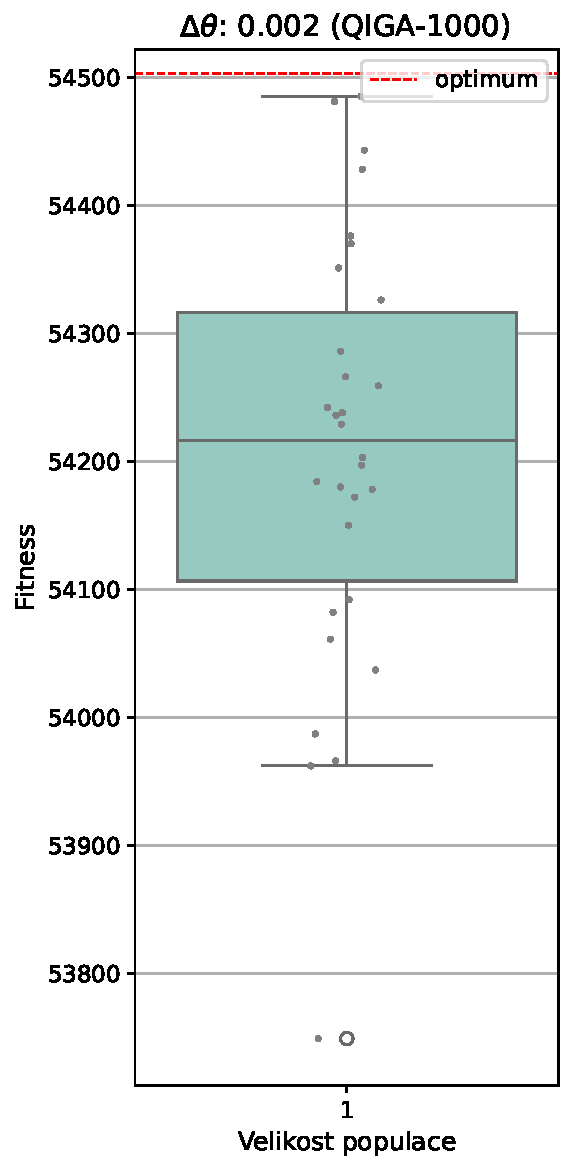
\includegraphics[width=\linewidth]{qiga/boxplot_qiga_1000_theta_0.002.pdf}
    \end{subfigure}
    \hfill
    \begin{subfigure}[b]{0.24\textwidth}
        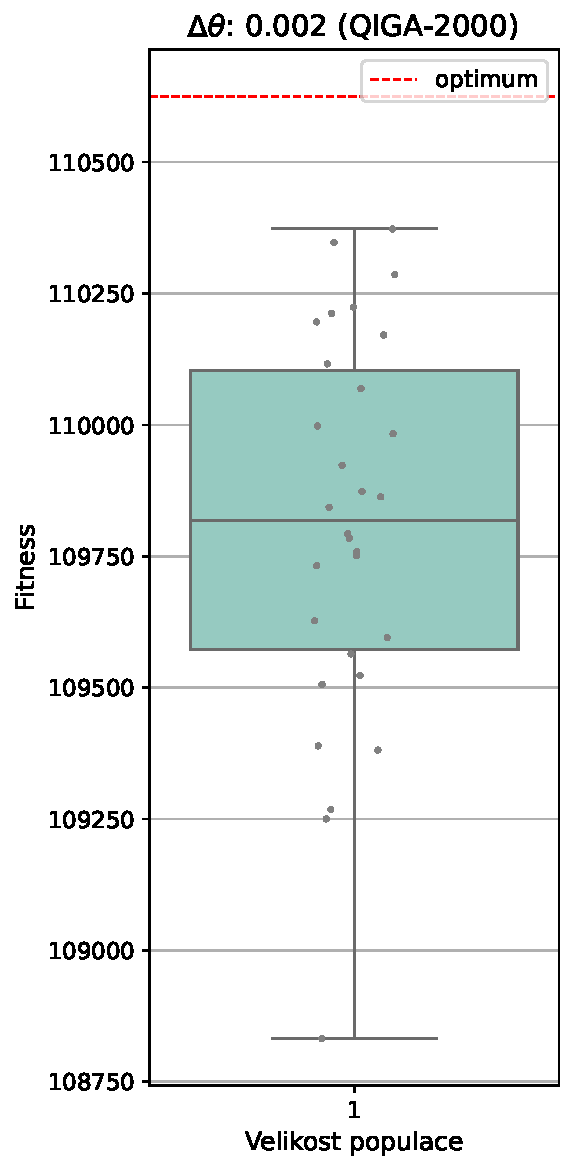
\includegraphics[width=\linewidth]{qiga/boxplot_qiga_2000_theta_0.002.pdf}
    \end{subfigure}
    \hfill
    \begin{subfigure}[b]{0.24\textwidth}
        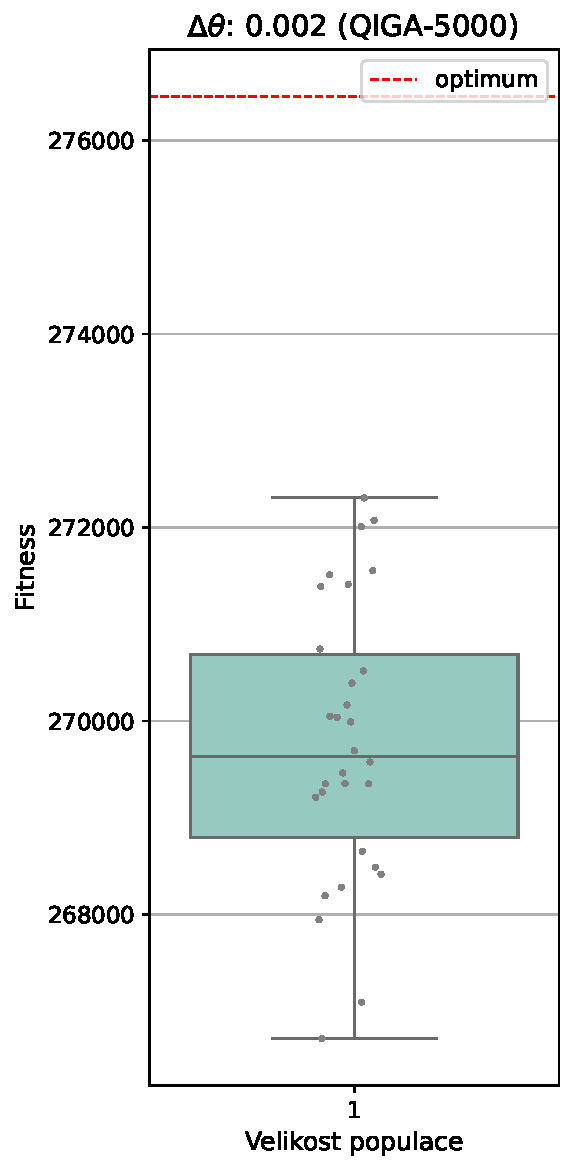
\includegraphics[width=\linewidth]{qiga/boxplot_qiga_5000_theta_0.002.pdf}
    \end{subfigure}
    \hfill
    \begin{subfigure}[b]{0.24\textwidth}
        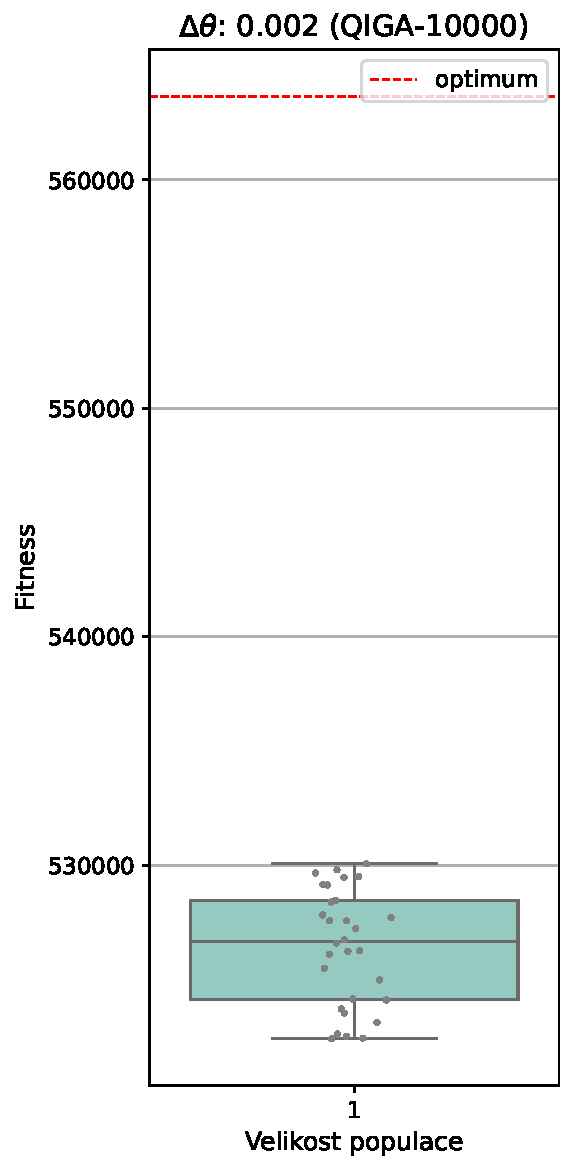
\includegraphics[width=\linewidth]{qiga/boxplot_qiga_10000_theta_0.002.pdf}
    \end{subfigure}
  
    \caption{Porovnání kvality řešení při hodnotě $\Delta\theta = 0{,}002$ a jednočlenné populaci na velkých instancích problému. Data prezentovaná na grafu byla získána algoritmem \emph{QIGA} na instancích, po řadě, velikosti 1\,000, 2\,000, 5\,000 a 10\,000 pomocí 30 nezávislých běhů s~10\,000 evaluacemi na běh.}
    \label{fig:qiga-large}
\end{figure}

Obrázek~\ref{fig:qiga-large} shrnuje výsledky experimentů provedených na rozsáhlejších instancích problému batohu, při doladěné hodnotě parametru $\Delta\theta = 0{,}002$. 
Z výsledků je patrné, že u~instancí o velikosti 1\,000 a 2\,000 se algoritmus \emph{QIGA} stále dokáže přiblížit k optimálnímu řešení. 
Naopak u větších instancí, konkrétně pro $5\,000$ a $10\,000$ položek batohu, dochází k~poklesu kvality řešení, což lze přičíst pevně nastavenému počtu evaluací. 

\begin{figure}[ht!]
    \centering
    \begin{subfigure}[b]{0.48\textwidth}
      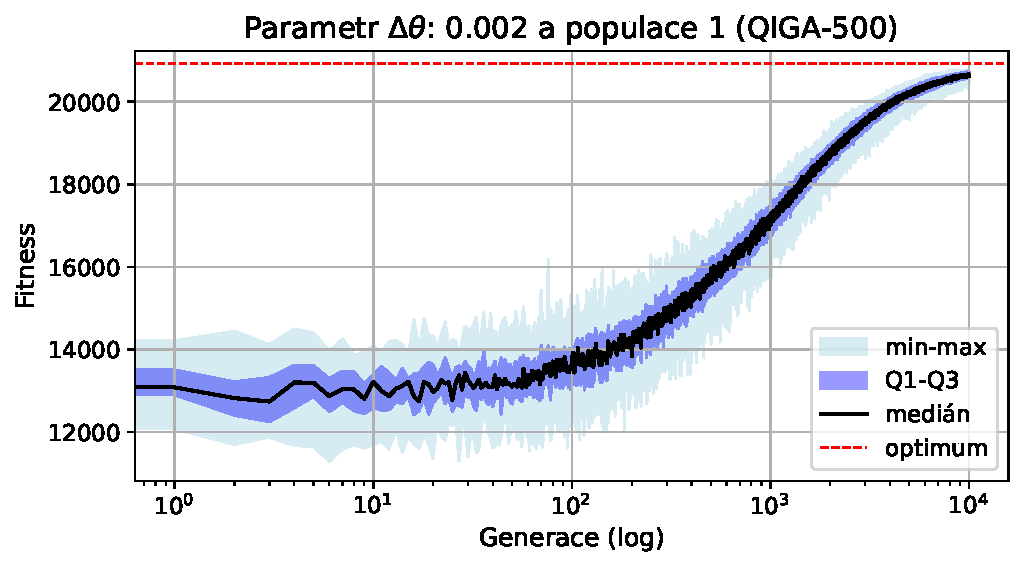
\includegraphics[width=\linewidth]{qiga/qiga_convergence_500_theta_0.002_population_1.pdf}
    \end{subfigure}
    \hfill
    \begin{subfigure}[b]{0.48\textwidth}
        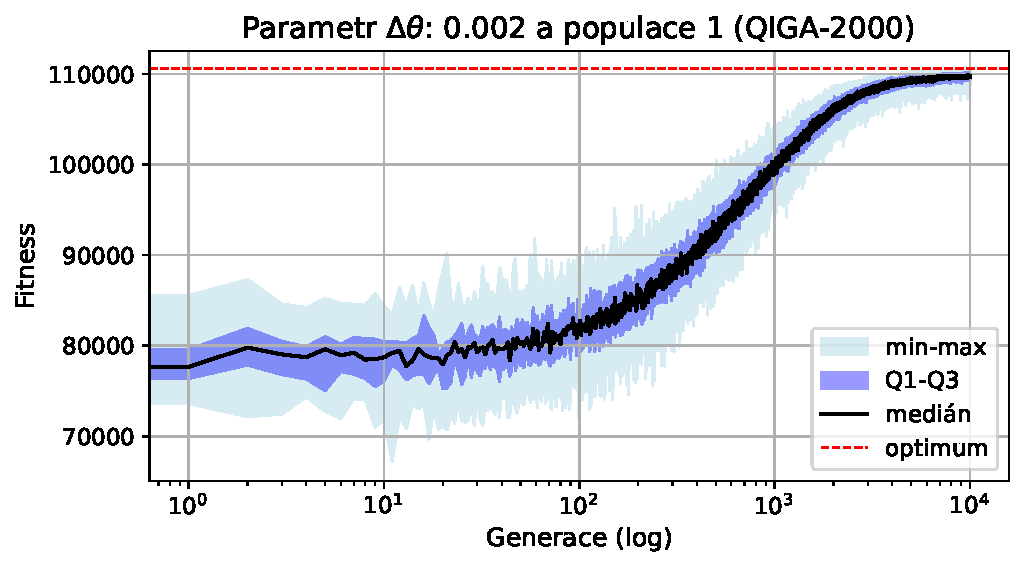
\includegraphics[width=\linewidth]{qiga/qiga_convergence_2000_theta_0.002_population_1.pdf}
    \end{subfigure}
    \caption{Konvergenční křivky pro $\Delta\theta = 0{,}002$ a jednočlennou populaci. Data prezentovaná na grafu byla získána algoritmem \emph{QIGA} na instancích, po řadě, velikosti 500 a 2\,000 pomocí 30 nezávislých běhů s 10\,000 evaluacemi na běh.}
    \label{fig:qiga-convergence}
\end{figure}

Obrázek~\ref{fig:qiga-convergence} zachycuje rychlost konvergence při velikostech instancí 500 a 2\,000. 
V obou případech byla použita jednočlenná populace a doladěná hodnota parametru $\Delta\theta = 0{,}002$.

\begin{table}[ht!]
    \centering
    \begin{tabular}{c c c c c c c c}
        \toprule
        \multirow{2}{*}{\centering$\boldsymbol{\Delta\theta}$\rule{0pt}{3.0ex}} & \multicolumn{7}{c}{\textbf{Instance}} \\
        \cmidrule(lr){2-8}
              & \textbf{100}    & \textbf{250}     & \textbf{500}     & \textbf{1\,000}  & \textbf{2\,000}   & \textbf{5\,000}   & \textbf{10\,000}  \\
        \midrule
        0,002 & 3\,967 & 10\,411 & 20\,760 & 54\,485 & 110\,373 & 272\,306 & 530\,066 \\
        0,01  & 3\,967 & 10\,402 & 20\,199 &         &          &          &          \\
        0,05  & 3\,919 & 9\,541  & 17\,762 &         &          &          &          \\
        0,1   & 3\,967 & 9\,986  & 18\,453 &         &          &          &          \\
        0,2   & 3\,965 &         &         &         &          &          &          \\
        0,5   & 3\,618 &         &         &         &          &          &          \\
        1,0   & 3\,603 &         &         &         &          &          &          \\
        2,0   & 3\,544 &         &         &         &          &          &          \\
        \midrule
        Optimum & 3\,967 & 10\,424 & 20\,925 & 54\,503 & 110\,625 & 276\,457 & 563\,647 \\
        \bottomrule
    \end{tabular}
    \caption{Nejlepší dosažené fitness hodnoty algoritmem \emph{QIGA} pro prezentované hodnoty parametru \(\Delta\theta\) a velikosti instancí.}
    \label{tab:qiga-theta-best}
\end{table}

Tabulka~\ref{tab:qiga-theta-best} prezentuje nejlepší dosažené fitness hodnoty řešení pro různé velikosti instancí a~hodnoty parametru $\Delta\theta$. 
Z výsledků je patrné, že nejnižší hodnota $\Delta\theta = 0{,}002$ vedla napříč instancemi k nejkvalitnějším řešením, přičemž u instance velikosti 100 bylo dokonce dosaženo optimálního řešení, zatímco u ostatních instancí se nejlepší nalezené hodnoty pohybovaly velmi blízko optimu. 

\section{Kvantově inspirované simulované žíhání}\label{sec:exp-qisa}
V této sekci jsou prezentovány výsledky experimentů zaměřených na kvantově inspirovaného simulovaného žíhání (\emph{QISA}). 
Cílem experimentů bylo analyzovat vliv různých konfigurací zahřívací funkce, chladicího plánu a míry ochlazování na kvalitu nalezených řešení. 
Konkrétní nastavení použitých hodnot parametrů je uvedeno v tabulce~\ref{tab:qisa-all-instances}. 

V první fázi experimentů byla provedeno ladění parametrů na menších instancí problému s cílem nalézt optimální konfiguraci algoritmu. 
Následně byl algoritmus s doladěnými hodnotami parametrů aplikován na větší instance problému s účelem ověřit jeho výkonnost při řešení náročnějších úloh. 

Na obrázku~\ref{fig:qisa-fining} jsou znázorněny výsledky experimentů pro různá nastavení zahřívací funkce a chladicího plánu, který využívají parametr míry ochlazování, přičemž grafy zobrazují výsledky pro instance problému o velikostech 100 a 500. 
Z výsledků je patrné, že míra ochlazování nemá výrazný vliv na kvalitu nalezených řešení a obdobně ani volba zahřívacího plánu zásadně neovlivňuje kvalitu výsledků. 

Výsledky experimentů s chladicími plány, jež nevyužívají parametr míry ochlazování, jsou zobrazeny na obrázku~\ref{fig:qisa-boxplot}. 
Z výsledků na uvedeném grafu je patrné, že logaritmický chladicí plán dosahuje výrazně horších výsledků ve srovnání s rekurzivně-logaritmickým plánem.

Z dat v tabulce~\ref{tab:qisa-low-max-values} je patrné, že většina kombinací parametrů dosahuje srovnatelných hodnot fitness, přičemž rozdíly mezi různými zahřívacími funkcemi a mírami ochlazování jsou minimální. 
Výrazně horších výsledků dosahuje pouze logaritmický chladicí plán, jenž ve všech velikostech instancí poskytuje nejnižší kvalitu řešení. 
Na základě těchto výsledků bylo pro další experimenty na větších instancích zvoleno nastavení s rekurzivně-logaritmickým chladicím plánem a sigmoidní zahřívací funkcí, jelikož tato kombinace dosáhla nejlepšího výsledku pro největší testovanou instanci.

\begin{figure}[ht!]
    \centering
    \begin{subfigure}[b]{\linewidth}
        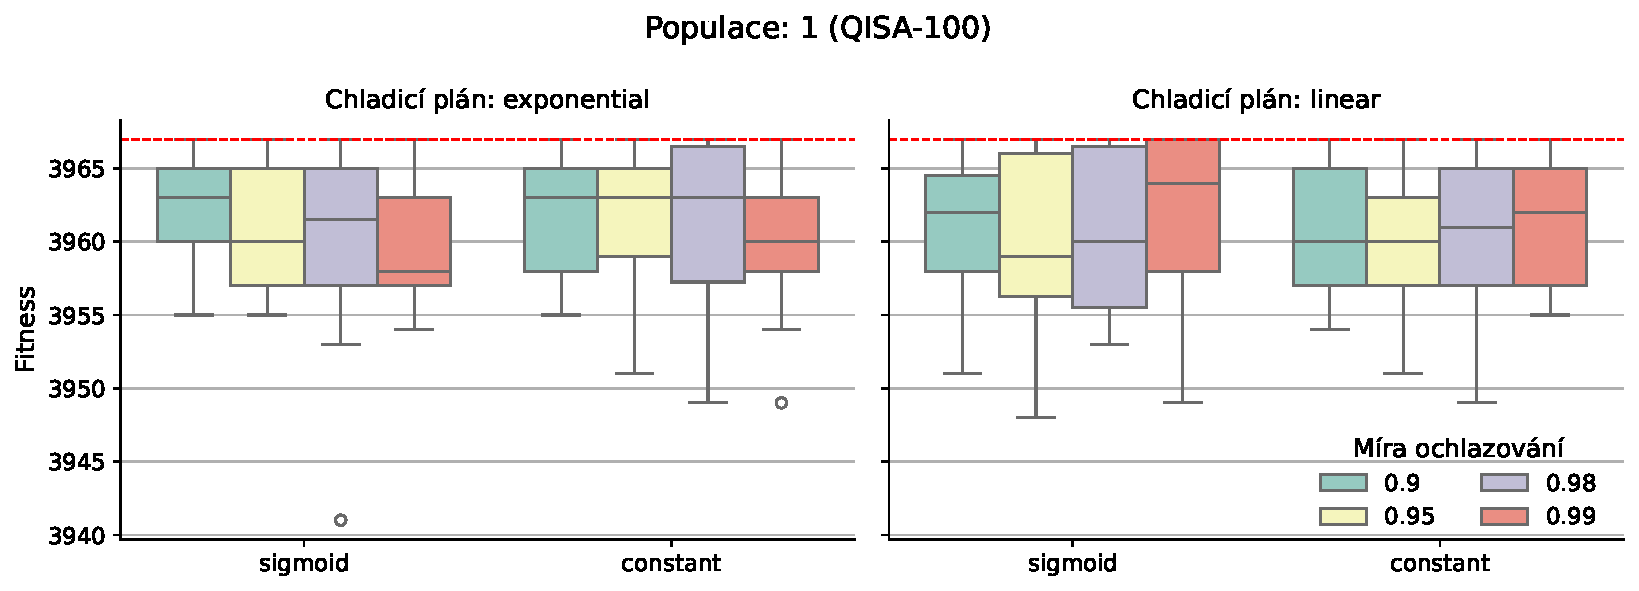
\includegraphics[width=\textwidth]{qisa/facet_boxplot_qisa_100_population_1.pdf}
    \end{subfigure}
    \begin{subfigure}[b]{\linewidth}
        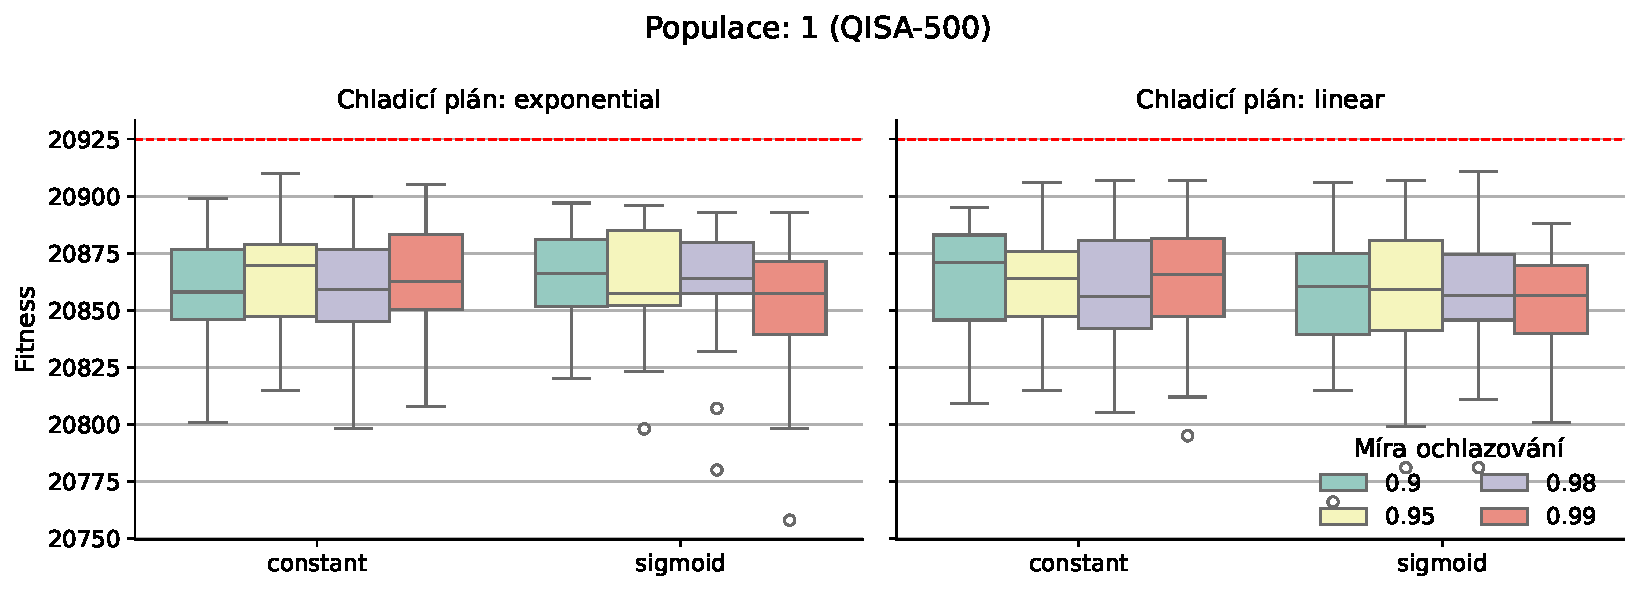
\includegraphics[width=\textwidth]{qisa/facet_boxplot_qisa_500_population_1.pdf}
    \end{subfigure}
    \caption{Porovnání vlivu různých zahřívacích funkcí a chladicích plánů pro různé míry ochlazování při jednočlenné populaci. Data prezentovaná na grafu byla získána algoritmem \emph{QISA} na instancích, po řadě, velikosti 100 a 500 pomocí 30 nezávislých běhů s 10\,000 evaluacemi na běh pro každou kombinaci prezentovaných parametrů.}
    \label{fig:qisa-fining}
\end{figure}

\begin{figure}[ht!]
    \centering
    \begin{subfigure}[b]{0.48\linewidth}
        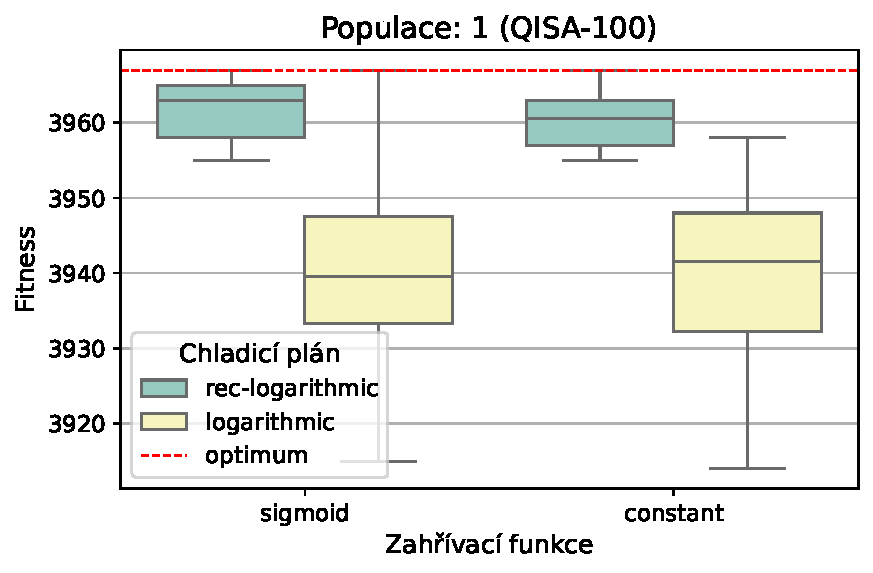
\includegraphics[width=\textwidth]{qisa/boxplot_qisa_100_population_1.pdf}
    \end{subfigure}
    \hfill
    \begin{subfigure}[b]{0.48\linewidth}
        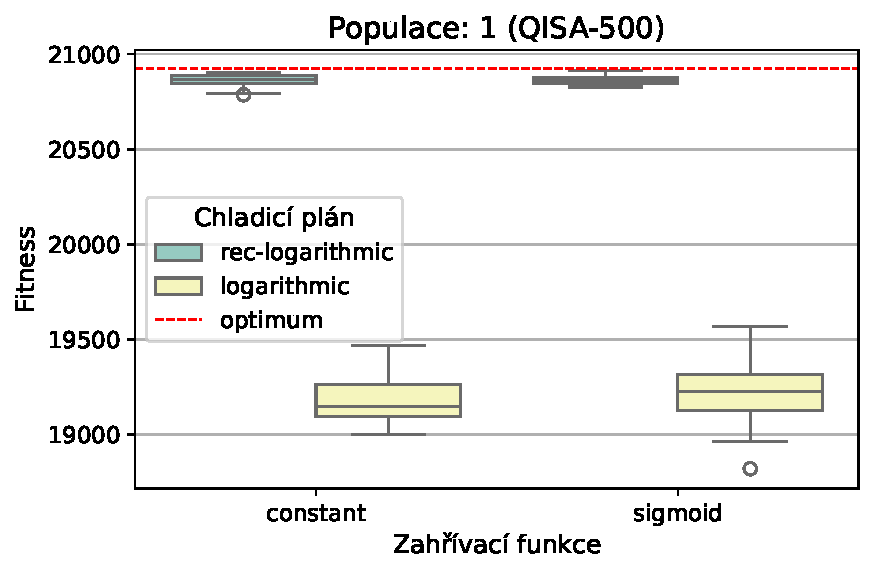
\includegraphics[width=\textwidth]{qisa/boxplot_qisa_500_population_1.pdf}
    \end{subfigure}
    \caption{Porovnání vlivu různých chladicích plánů a zahřívacích funkcí, jenž nevyužívají parametr míry ochlazování. Data prezentovaná na grafu byla získána algoritmem \emph{QISA} na instancích, po řadě, velikosti 100 a 500 pomocí 30 nezávislých běhů s 10\,000 evaluacemi na běh pro každou kombinaci prezentovaných parametrů.}
    \label{fig:qisa-boxplot}
\end{figure}

\begin{table}[ht!]
    \centering
    \begin{tabular}{c c c c c c}
        \toprule
        \multirow{2}{*}{\makecell{\textbf{Chladicí}\\\textbf{plán}}} & \multirow{2}{*}{\makecell{\textbf{Zahřívací}\\\textbf{funkce}}} & \multirow{2}{*}{\makecell{\textbf{Míra}\\\textbf{ochlazování}}} & \multicolumn{3}{c}{\textbf{Instance}} \\
        \cmidrule(lr){4-6}
         &  &  & \textbf{100}    & \textbf{250}     & \textbf{500}\\
        \midrule
        exp & konstantní & 0,9  & 3\,967 & 10\,421 & 20\,899 \\
        exp & konstantní & 0,95 & 3\,967 & 10\,421 & 20\,910 \\
        exp & konstantní & 0,98 & 3\,967 & 10\,420 & 20\,900 \\
        exp & konstantní & 0,99 & 3\,967 & 10\,421 & 20\,905 \\
        exp & sigmoidní  & 0,9  & 3\,967 & 10\,419 & 20\,897 \\
        exp & sigmoidní  & 0,95 & 3\,967 & 10\,420 & 20\,896 \\
        exp & sigmoidní  & 0,98 & 3\,967 & 10\,421 & 20\,893 \\
        exp & sigmoidní  & 0,99 & 3\,967 & 10\,420 & 20\,893 \\
        lin & konstantní & 0,9  & 3\,967 & 10\,421 & 20\,895 \\
        lin & konstantní & 0,95 & 3\,967 & 10\,420 & 20\,906 \\
        lin & konstantní & 0,98 & 3\,967 & 10\,422 & 20\,907 \\
        lin & konstantní & 0,99 & 3\,967 & 10\,421 & 20\,907 \\
        lin & sigmoidní  & 0,9  & 3\,967 & 10\,421 & 20\,906 \\
        lin & sigmoidní  & 0,95 & 3\,967 & 10\,421 & 20\,907 \\
        lin & sigmoidní  & 0,98 & 3\,967 & 10\,420 & 20\,911 \\
        lin & sigmoidní  & 0,99 & 3\,967 & 10\,420 & 20\,888 \\
        log & konstantní & ---  & 3\,958 & 10\,201 & 19\,469 \\
        log & sigmoidní  & ---  & 3\,967 & 10\,221 & 19\,567 \\
        rec-log & konstantní & --- & 3\,967 & 10\,420 & 20\,905 \\
        rec-log & sigmoidní  & --- & 3\,967 & 10\,420 & 20\,916 \\
        \midrule
        \multicolumn{3}{c}{Optimum} & 3\,967 & 10\,424 & 20\,925  \\
        \bottomrule
    \end{tabular}
    \caption{Nejlepší dosažené fitness hodnoty algoritmem \emph{QISA} pro prezentované kombinace nastavení chladicího plánu, zahřívací funkce a míry ochlazování při malých instancích problému.}
    \label{tab:qisa-low-max-values}
\end{table}

\begin{figure}[ht!]
    \centering
    \begin{subfigure}[b]{0.24\textwidth}
      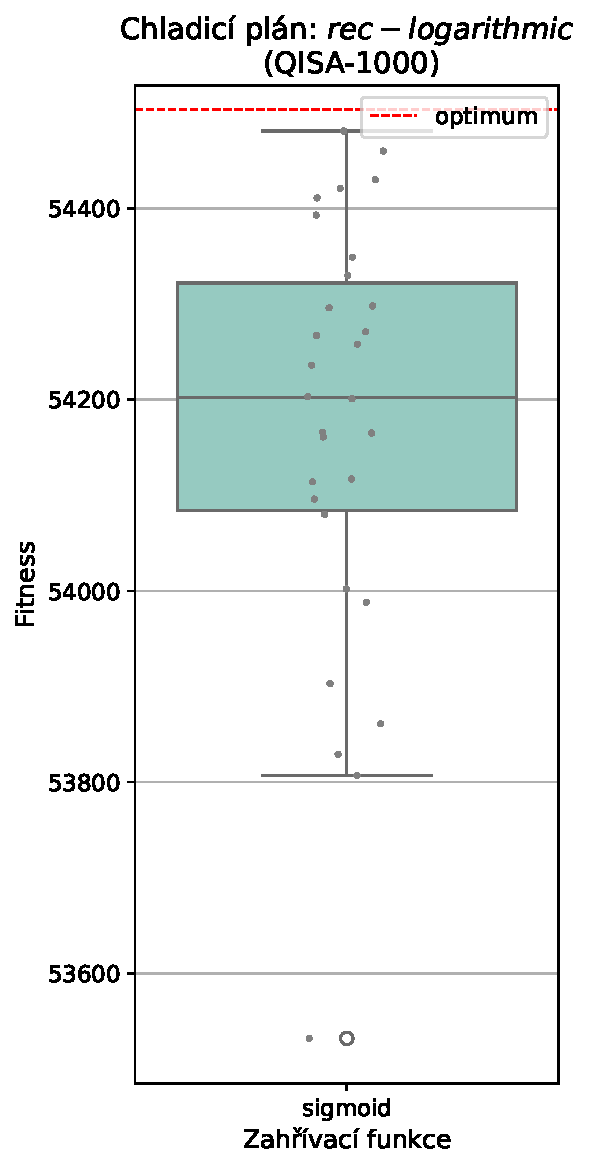
\includegraphics[width=\linewidth]{qisa/boxplot_qisa_1000_large.pdf}
    \end{subfigure}
    \hfill
    \begin{subfigure}[b]{0.24\textwidth}
        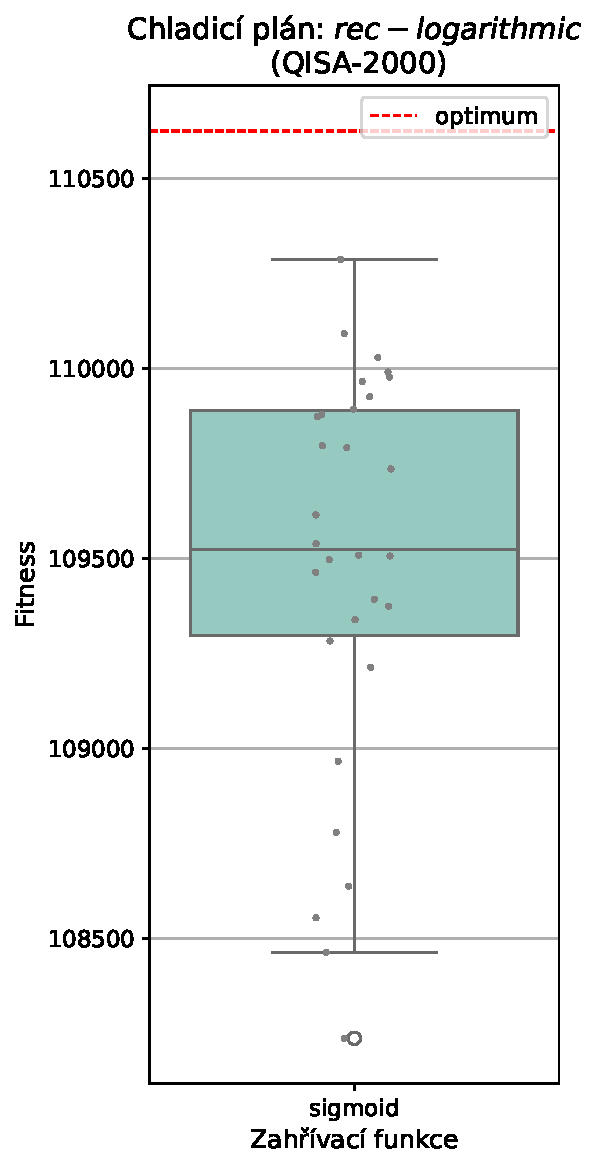
\includegraphics[width=\linewidth]{qisa/boxplot_qisa_2000_large.pdf}
    \end{subfigure}
    \hfill
    \begin{subfigure}[b]{0.24\textwidth}
        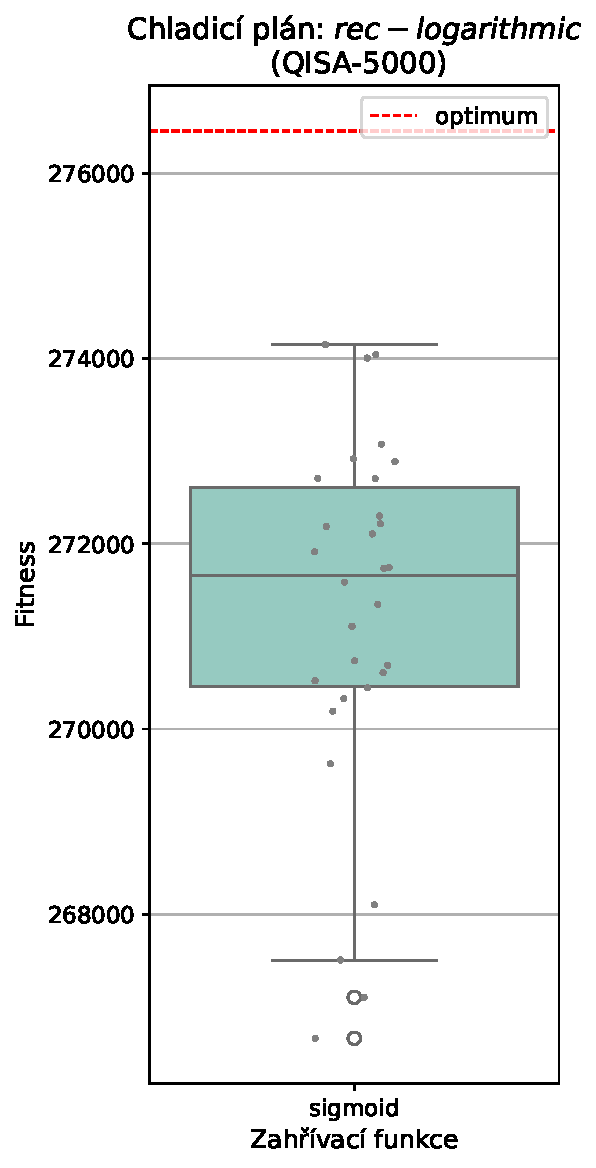
\includegraphics[width=\linewidth]{qisa/boxplot_qisa_5000_large.pdf}
    \end{subfigure}
    \hfill
    \begin{subfigure}[b]{0.24\textwidth}
        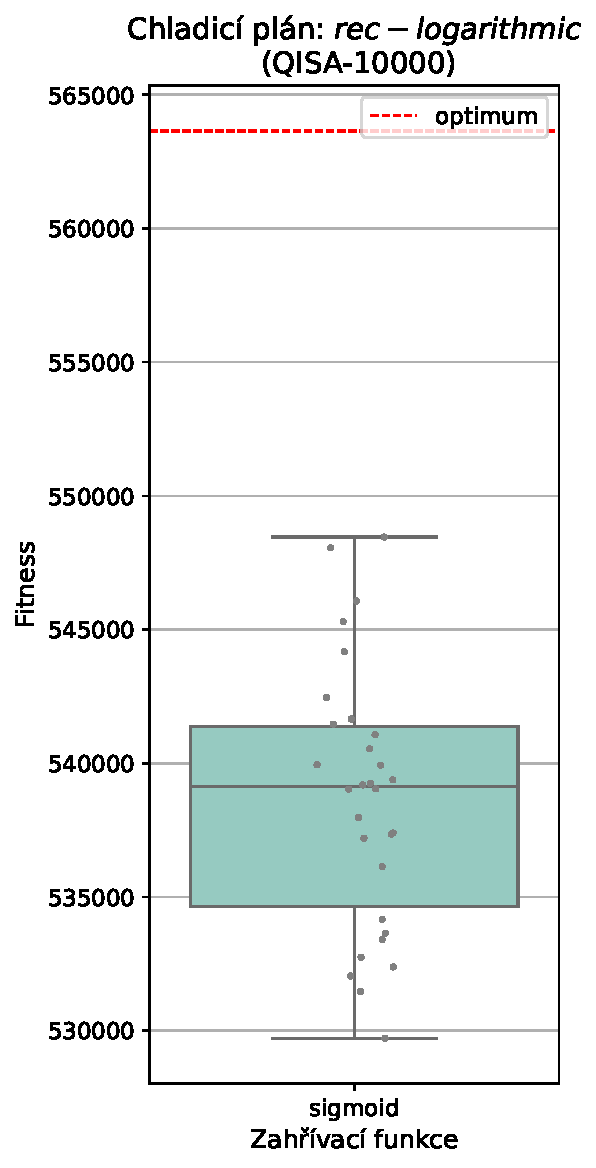
\includegraphics[width=\linewidth]{qisa/boxplot_qisa_10000_large.pdf}
    \end{subfigure}
    \caption{Porovnání kvality nalezených řešení při rekurzivně-logaritmickém chladicím plánu, sigmoidní zahřívací funkci při velkých instancích problému a jednočlenné populaci. Data prezentovaná na grafu byla získána algoritmem \emph{QISA} na instancích, po řadě, velikosti 1\,000, 2\,000, 5\,000 a 10\,000 pomocí 30 nezávislých běhů s 10\,000 evaluacemi na běh.}
    \label{fig:qisa-large}
\end{figure}

Na obrázku~\ref{fig:qisa-large} jsou prezentovány výsledky experimentů provedených na velkých instancí problému při konfiguraci algoritmu využívající rekurzivně-logaritmický chladicí plán a sigmoidní zahřívací funkci. 
Z grafů je patrné, že i při velkých instancí problému (1\,000, 2\,000 a 5\,000) si algoritmus udržuje výsledky blízko optimu. 
Výraznější pokles kvality řešení je patrný až u instance velikosti 10\,000, kde algoritmus, již nedosahuje kvalitních výsledků. 
Výsledky dosažené tímto nastavením jsou dále detailněji uvedeny v~tabulce~\ref{tab:qisa-high-max-values}. 

\begin{table}[ht!]
    \centering
    \begin{tabular}{c c c c c c c}
        \toprule
        \multirow{2}{*}{\makecell{\textbf{Chladicí}\\\textbf{plán}}} & \multirow{2}{*}{\makecell{\textbf{Zahřívací}\\\textbf{funkce}}} & \multicolumn{4}{c}{\textbf{Instance}} \\
        \cmidrule(lr){3-6}
         &  & \textbf{1\,000}    & \textbf{2\,000}     & \textbf{5\,000} & \textbf{10\,000}\\
        \midrule
        rec-log & sigmoidní  & 54\,481 & 110\,287 & 274\,150 & 548\,460 \\
        \midrule
        \multicolumn{2}{c}{Optimum} & 54\,503 & 110\,625 & 276\,457 & 563\,647  \\
        \bottomrule
    \end{tabular}
    \caption{Nejlepší dosažené fitness hodnoty algoritmem \emph{QISA} pro prezentované nastavení při velkých instancích problému.}
    \label{tab:qisa-high-max-values}
\end{table}

Obrázek~\ref{fig:qiga-convergence} zachycuje průběhy zlepšování fitness algoritmu \emph{QISA} při řešení instancí problému o velikosti 500 a~2\,000. 
V obou případech byla použita jednočlenná populace spolu s rekurzivně-logaritmický chladicí plánem a~sigmodiní zahřívací funkcí.

\begin{figure}[ht!]
    \centering
    \begin{subfigure}[b]{0.48\textwidth}
      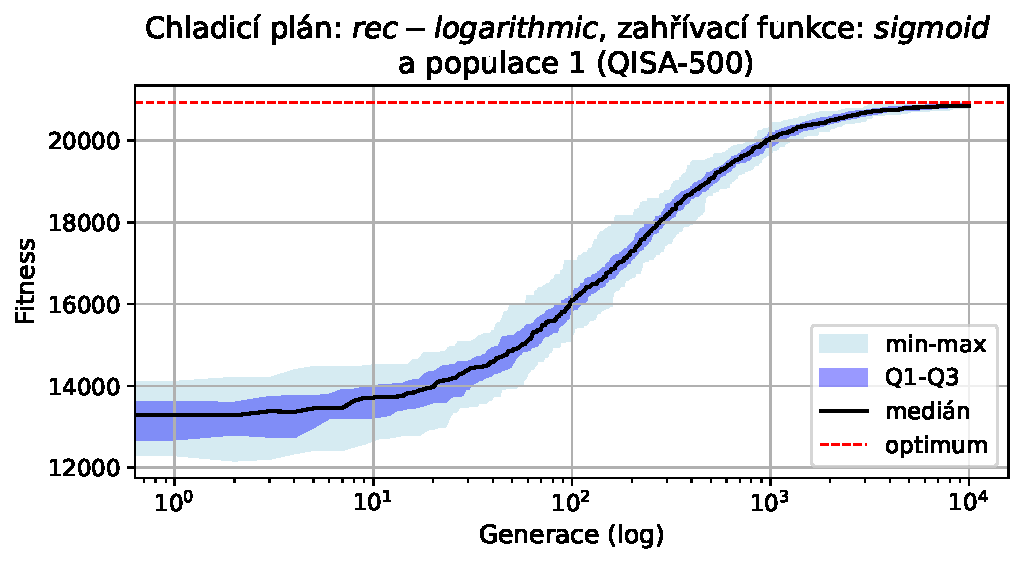
\includegraphics[width=\linewidth]{qisa/qisa_convergence_500_cooling_rec-logarithmic_observation_sigmoid_population_1.pdf}
    \end{subfigure}
    \hfill
    \begin{subfigure}[b]{0.48\textwidth}
        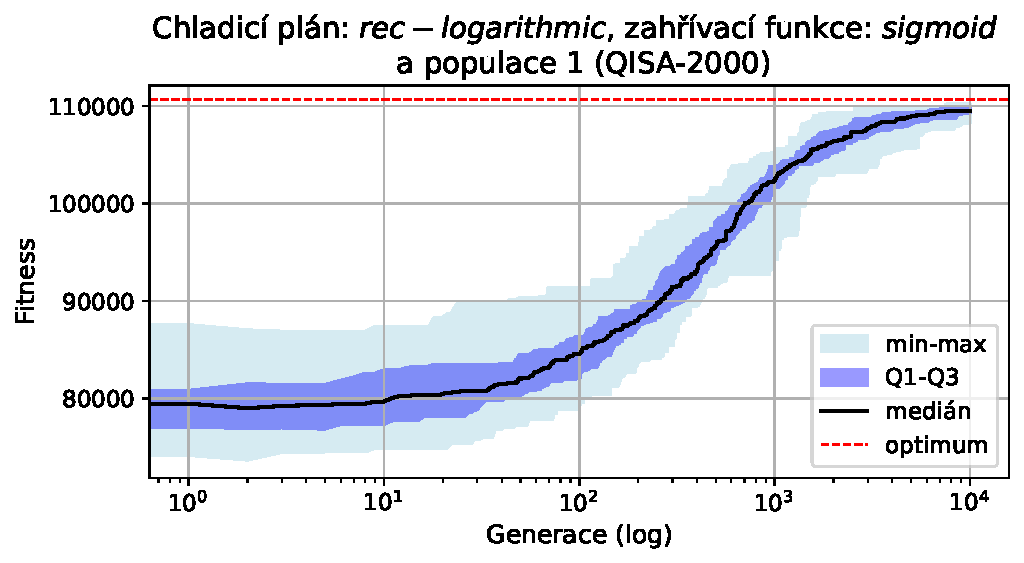
\includegraphics[width=\linewidth]{qisa/qisa_convergence_2000_cooling_rec-logarithmic_observation_sigmoid_population_1.pdf}
    \end{subfigure}
    \caption{Konvergenční křivky pro konfiguraci algoritmu, jež byla nastavena na rekurzivně-logaritmický chladicí plán a sigmoidní zahřívací funkci. Data prezentovaná na grafu byla získána algoritmem \emph{QISA} na instancích, po řadě, velikosti 500 a 2\,000 pomocí 30 nezávislých běhů s 10\,000 evaluacemi na běh.}
    \label{fig:qisa-convergence}
\end{figure}

\section{Kvantová evoluce roje}\label{sec:exp-qse}
V této sekci jsou prezentovány výsledky experimentů zaměřených na kvantovou evoluci roje (\emph{QSE}). 
Cílem experimentů bylo analyzovat vliv různých konfigurací počátečních rychlostí a~velikostí populací na kvalitu nalezených řešení. 
Na rozdíl od algoritmů \emph{QIGA} a \emph{QISA}, které nedisponují mechanismem vzájemné interakce jedinců, algoritmus \emph{QSE} již tento mechanismum využívá, což může mít vliv na průběh evoluce a výslednou kvalitu řešení. 
Z~tohoto důvodu bude při interpretaci výsledků kladen důraz právě na tyto aspekty.
Konkrétní nastavení použitých hodnot parametrů je uvedeno v tabulce~\ref{tab:qse-all-instances}. 

\begin{figure}[ht!]
    \centering
    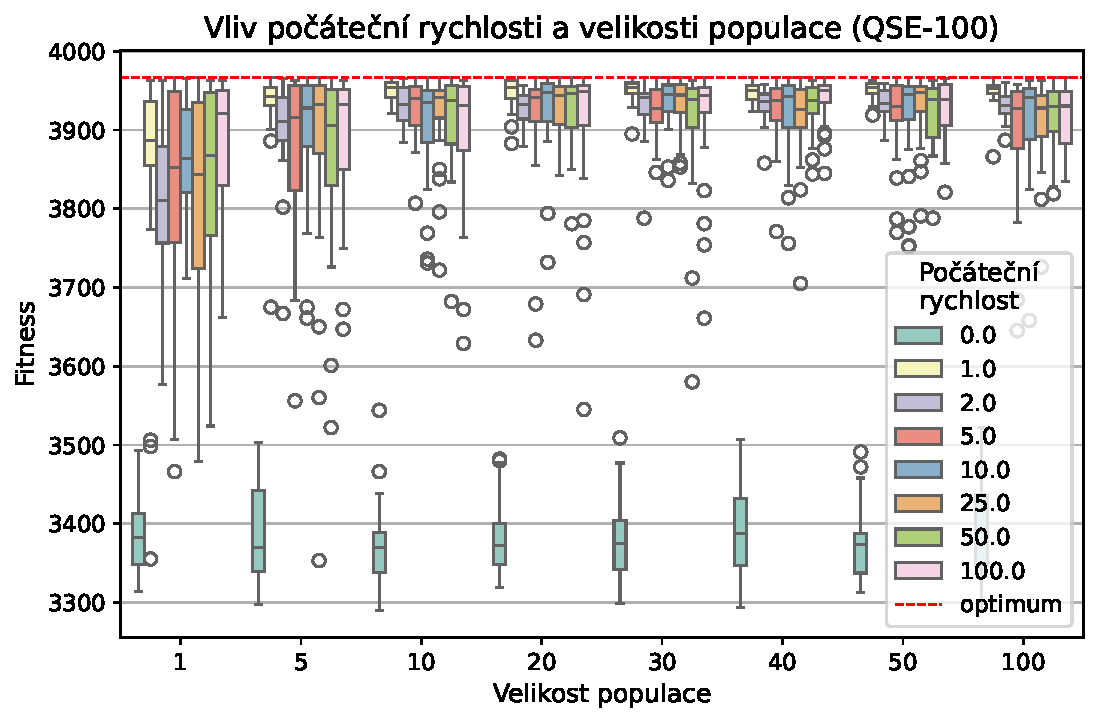
\includegraphics[width=0.98\textwidth]{qse/boxplot_qse_100_velocity.pdf}
    \caption{Porovnání vlivu různých velikostí populací a hodnot počátečních rychlostí na kvalitu řešení. Data prezentovaná na grafu byla získána algoritmem \emph{QSE} na instanci velikosti 100 pomocí 30 nezávislých běhů s 10\,000 evaluacemi na běh pro každou kombinaci prezentovaných parametrů.}
    \label{fig:qse-100-all}
\end{figure}

Z výsledků experimentů na instanci velikosti 100 na obrázku~\ref{fig:qse-100-all} je patrné, že nejstabilnější a zároveň nejkvalitnější výsledky poskytuje hodnota počáteční rychlosti 1, zatímco nulová počáteční rychlost generuje nejméně kvalitní výsledky. 

\begin{figure}[ht!]
    \centering
    \begin{subfigure}[b]{0.45\textwidth}
      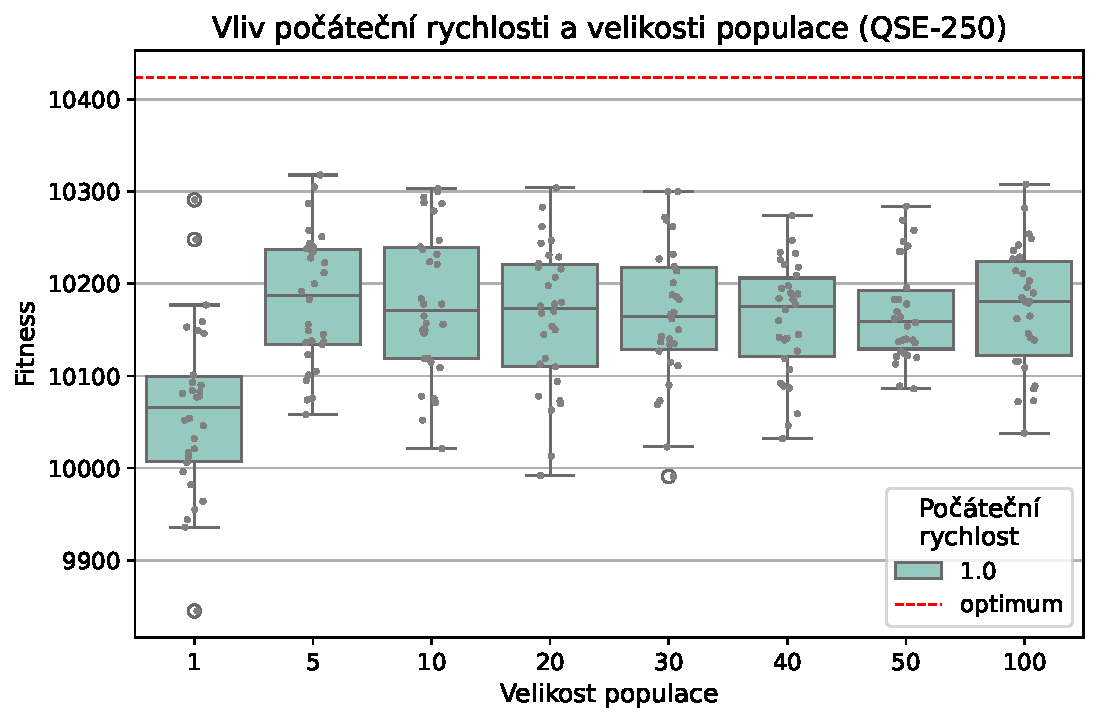
\includegraphics[width=\linewidth]{qse/boxplot_qse_250_velocity_filtered.pdf}
    \end{subfigure}
    \hfill
    \begin{subfigure}[b]{0.48\textwidth}
        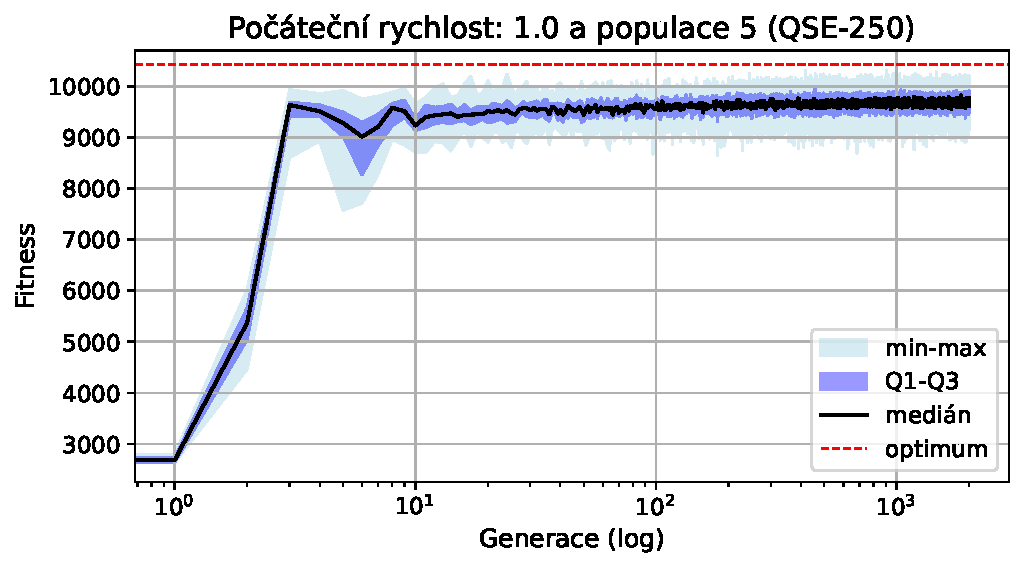
\includegraphics[width=\linewidth]{qse/qse_convergence_250_velocity_1.0_population_5.pdf}
    \end{subfigure}
    \caption{Výsledky experimentů algoritmu \emph{QSE} na instanci velikosti 250. Vlevo jsou znázorněny krabicové grafy dosažených hodnot fitness pro různé velikosti populace při počáteční rychlosti 1, vpravo pak konvergenční křivka vývoje fitness při populaci čítající 5 jedinců a počáteční rychlosti 1. Data byla získána pomocí 30 nezávislých běhů s 10\,000 evaluacemi na běh pro každou kombinaci prezentovaných parametrů.}
    \label{fig:qse-250-mix}
\end{figure}

Ze zobrazeného krabicového grafu na obrázku~\ref{fig:qse-250-mix} prezentujícího výsledky experimentů pro vybranou hodnotu počáteční rychlosti 1 je patrné, že velikost populace při instanci 250 nemá výrazný vliv na kvalitu nalezených řešení.
Zároveň lze z konvergenční křivky na stejném obrázku~\ref{fig:qse-250-mix} pozorovat, že algoritmus při pětičlenné populaci velmi rychle konverguje k~řešením blízkým optimu, přičemž další vývoj je již minimální. 
Z těchto důvodů byla pro experimenty na větších instancích zvolena právě pětičlenná populace, neboť umožňuje uplatnění mechanismu vzájemné komunikace jedinců a zároveň poskytuje jednotlivým jedincům dostatek prostoru pro jejich vývoj. 

Na obrázku~\ref{fig:qse-large} jsou uvedeny výsledky experimentů provedených na velkých instancích problému s konfigurací algoritmu nastavenou na počáteční rychlost 1 a pětičlennou populaci.
Z grafů a z tabulky nejvyšších dosažených hodnot fitness~\ref{tab:qse-high-max-values} je zřejmé, že při velikosti instance 1\,000 algoritmus dosáhl řešení velmi blízkého optimu. Se zvyšující se velikostí instance však docházelo k postupnému zhoršování kvality nalezených řešení.

\begin{figure}[ht!]
    \centering
    \begin{subfigure}[b]{0.24\textwidth}
      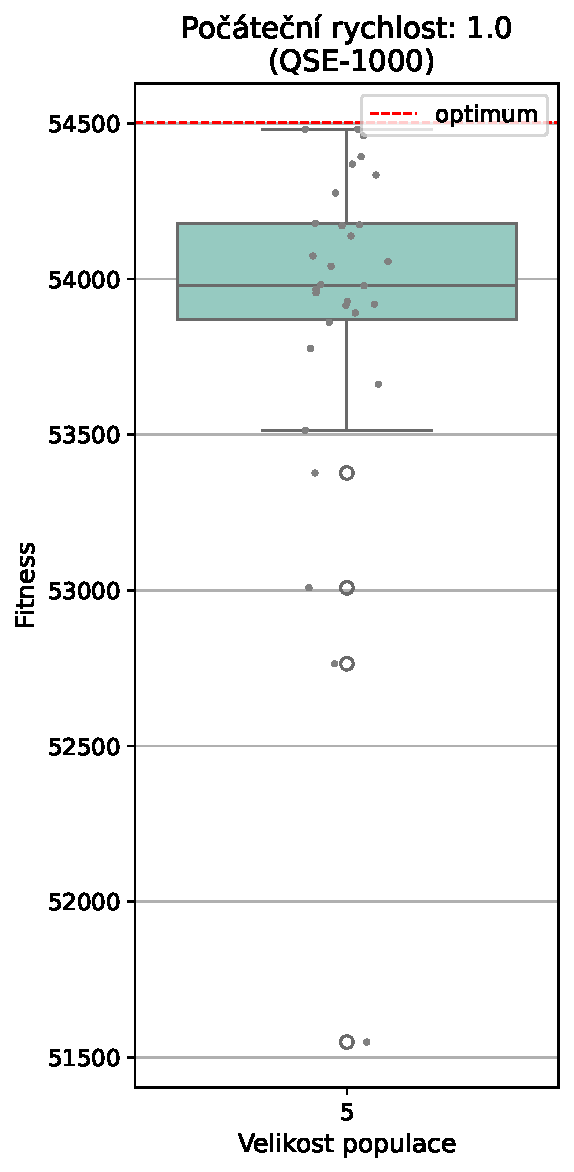
\includegraphics[width=\linewidth]{qse/boxplot_qse_1000_large.pdf}
    \end{subfigure}
    \hfill
    \begin{subfigure}[b]{0.24\textwidth}
        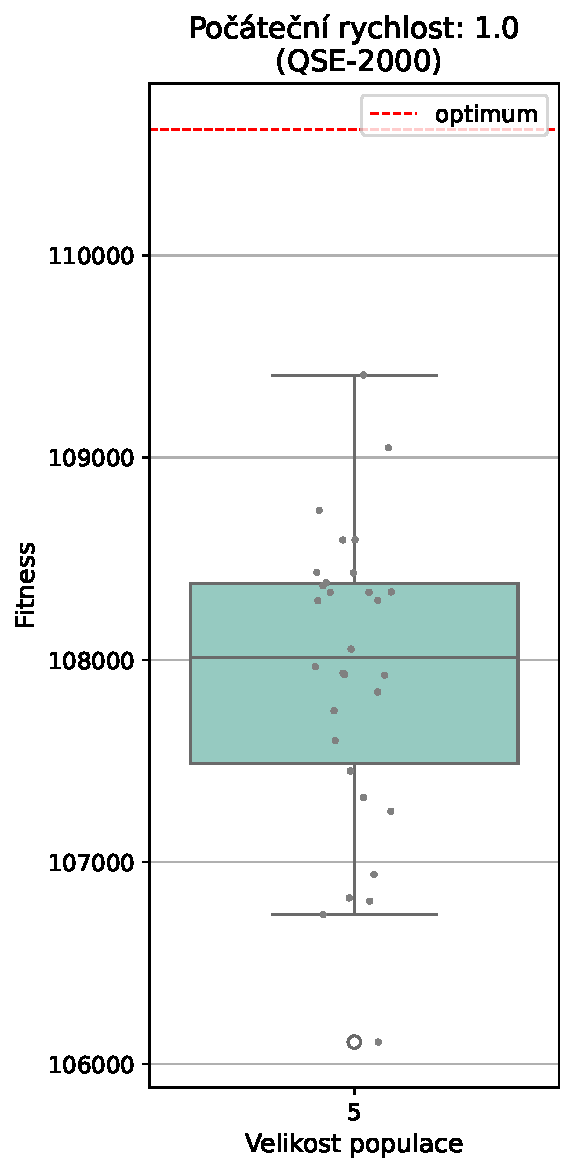
\includegraphics[width=\linewidth]{qse/boxplot_qse_2000_large.pdf}
    \end{subfigure}
    \hfill
    \begin{subfigure}[b]{0.24\textwidth}
        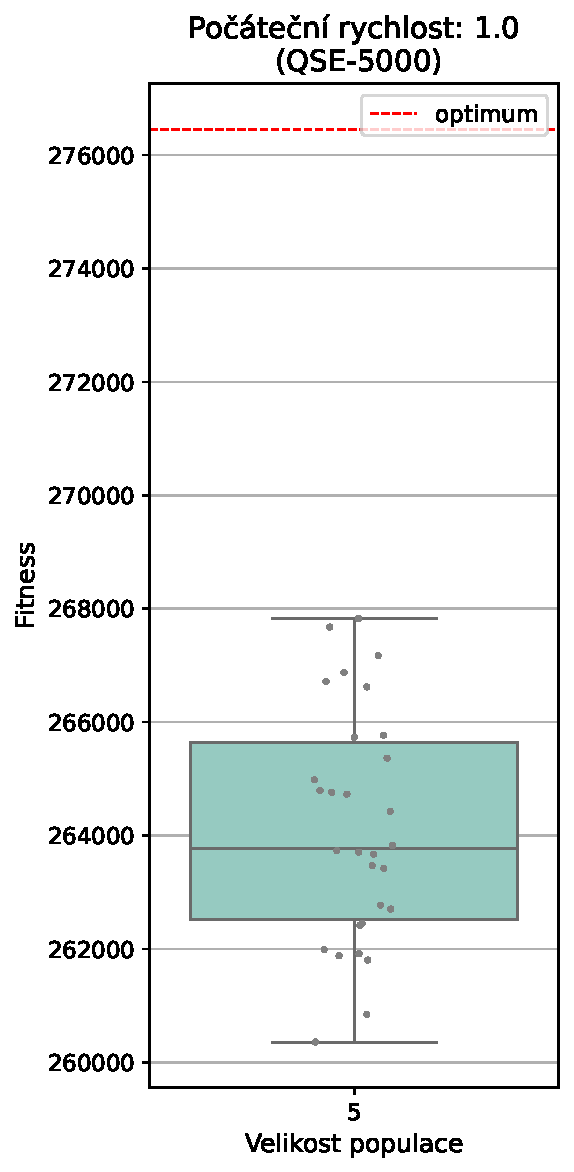
\includegraphics[width=\linewidth]{qse/boxplot_qse_5000_large.pdf}
    \end{subfigure}
    \hfill
    \begin{subfigure}[b]{0.24\textwidth}
        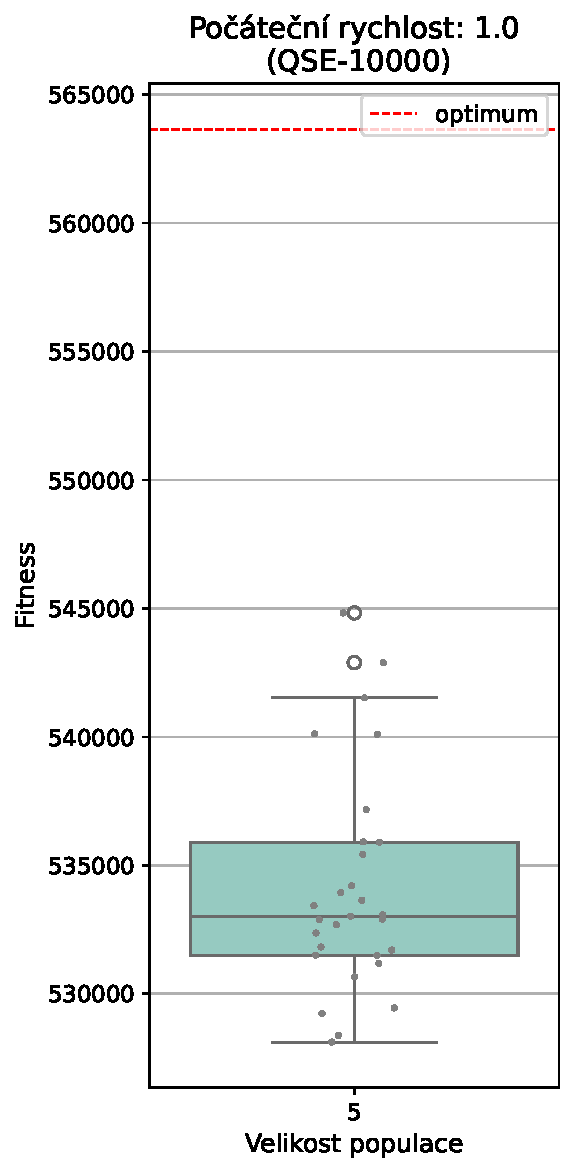
\includegraphics[width=\linewidth]{qse/boxplot_qse_10000_large.pdf}
    \end{subfigure}
    \caption{Porovnání kvality nalezených řešení při hodnotě počáteční rychlosti 1 a pětičlenné populaci při velkých instancích problému. Data prezentovaná na grafu byla získána algoritmem \emph{QSE} na instancích, po řadě, velikosti 1\,000, 2\,000, 5\,000 a 10\,000 pomocí 30 nezávislých běhů s 10\,000 evaluacemi na běh.}
    \label{fig:qse-large}
\end{figure}

\begin{table}[ht!]
    \centering
    \begin{tabular}{c c c c c c}
        \toprule
        \multirow{2}{*}{\makecell{\textbf{Počáteční}\\\textbf{rychlost}}} & \multicolumn{4}{c}{\textbf{Instance}} \\
        \cmidrule(lr){2-5}
         & \textbf{1\,000}    & \textbf{2\,000}     & \textbf{5\,000} & \textbf{10\,000}\\
        \midrule
        1  & 54\,481 & 108\,387 & 267\,827 & 544\,824 \\
        \midrule
        \multicolumn{1}{c}{Optimum} & 54\,503 & 110\,625 & 276\,457 & 563\,647  \\
        \bottomrule
    \end{tabular}
    \caption{Nejlepší dosažené fitness hodnoty algoritmem \emph{QSE} pro prezentované nastavení při velkých instancích problému při populaci čítající 5 jedinců.}
    \label{tab:qse-high-max-values}
\end{table}

Obrázek~\ref{fig:qse-convergence} zachycuje průběhy zlepšování fitness algoritmu při řešení instancí problému velikosti 500 a~2\,000. 
V obou případech byla použita pětičlenná populace spolu s počáteční rychlostí nastavenou na hodnotu 1.

\begin{figure}[ht!]
    \centering
    \begin{subfigure}[b]{0.48\textwidth}
      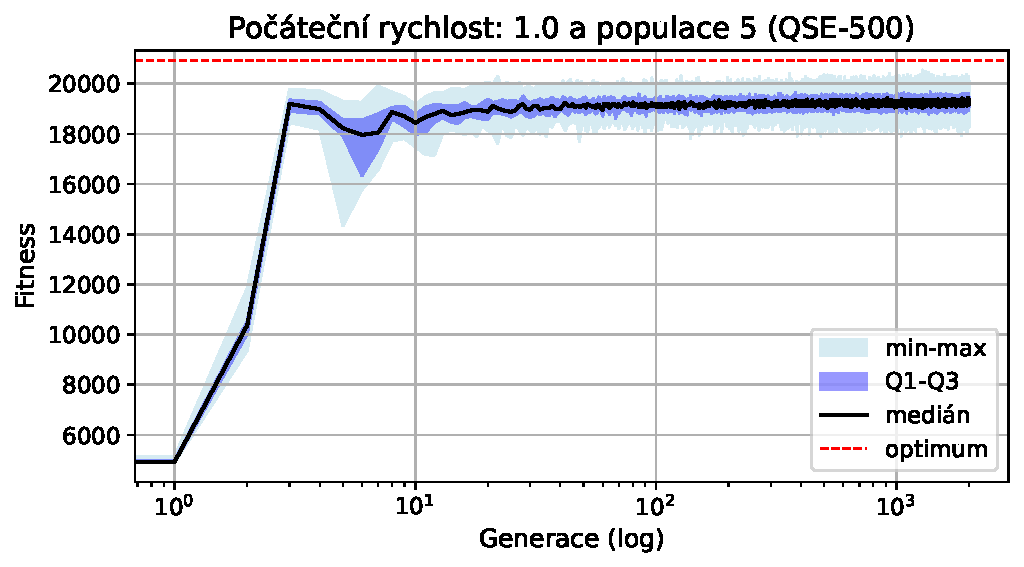
\includegraphics[width=\linewidth]{qse/qse_convergence_500_velocity_1.0_population_5.pdf}
    \end{subfigure}
    \hfill
    \begin{subfigure}[b]{0.48\textwidth}
        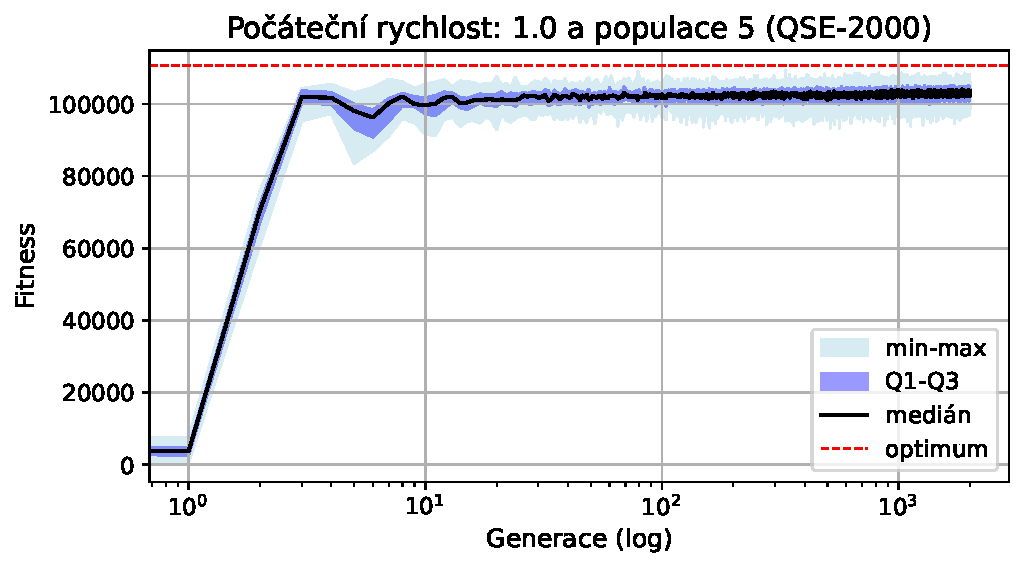
\includegraphics[width=\linewidth]{qse/qse_convergence_2000_velocity_1.0_population_5.pdf}
    \end{subfigure}
    \caption{Konvergenční křivky algoritmu, jehož parametr počáteční rychlosti byl nastaven na hodnotu 1 při pětičlenné populaci. Data prezentovaná na grafu byla získána algoritmem \emph{QSE} na instancích, po řadě, velikosti 500 a 2\,000 pomocí 30 nezávislých běhů s 10\,000 evaluacemi na běh.}
    \label{fig:qse-convergence}
\end{figure}

\section{Kvantově inspirovaná optimalizace rojem částic}\label{sec:exp-qipso}
V této sekci jsou prezentovány výsledky experimentů zaměřených na kvantově inspirovanou optimalizaci rojem částic (\emph{QIPSO}). 
Cílem experimentů bylo analyzovat vliv různých konfigurací počátečních rychlostí, kognitivních koeficientů, sociálních koeficientů, parametrů tření a~velikostí populací na kvalitu nalezených řešení. 
Obdobně jako algoritmus \emph{QSE} i algoritmus \emph{QIPSO} disponuje mechanismem vzájemné interakce jedinců. 
Konkrétní nastavení použitých hodnot parametrů je uvedeno v tabulce~\ref{tab:qipso-all-params}. 

\begin{figure}[ht!]
    \centering
    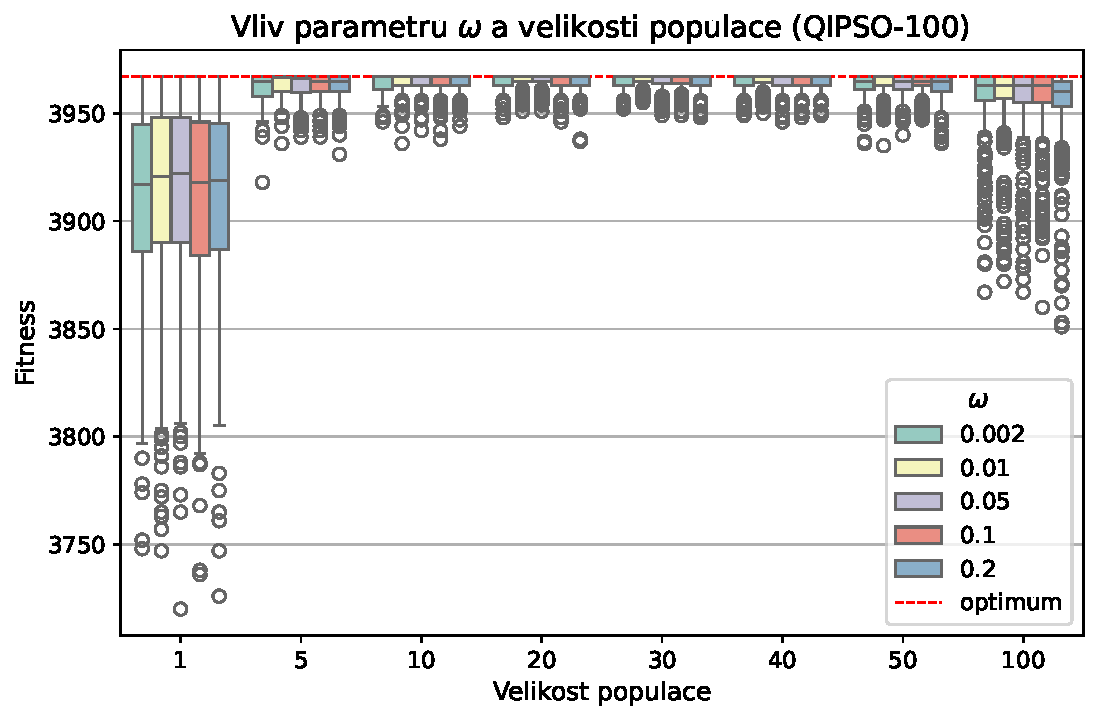
\includegraphics[width=0.96\textwidth]{qipso/boxplot_qipso_100_all_omega.pdf}
    \caption{Závislost kvality řešení na velikosti populace pro různé hodnoty parametru $\omega$. Data prezentovaná na grafu byla získána algoritmem \emph{QIPSO} na instanci velikosti 100 pomocí 30 nezávislých běhů s 10\,000 evaluacemi na běh pro každou kombinaci testovaných parametrů.}
    \label{fig:qipso-100-all-omega}
\end{figure}

Jak je patrné z obrázku \ref{fig:qipso-100-all-omega}, populace o velikosti 1 a 100 poskytují nekvalitní řešení, a proto budou v dalších grafech tyto velikosti vynechány, rovněž nebude dále uvažována populace 50, protože při experimentování s většími instancemi problémů by jednotlivci měli omezený prostor pro svůj rozvoj z důvodu omezeného počtu evaluací. 
Na základě těchto výsledků byly vybrány k další analýze hodnoty parametru $\omega$ $0{,}01$ a $0{,}05$, které průměrně dosahovaly kvalitnějších výsledků oproti ostatním testovaným hodnotám.

\begin{figure}
    \centering
    \begin{subfigure}[b]{0.48\textwidth}
        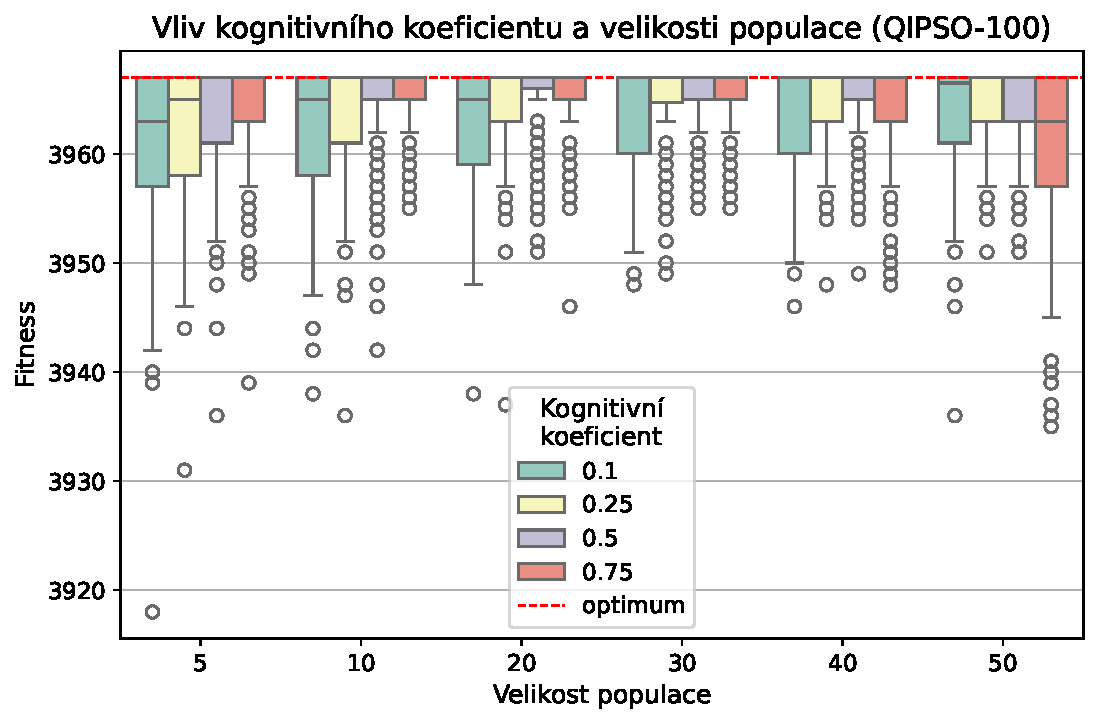
\includegraphics[width=\textwidth]{qipso/boxplot_qipso_100_all_cognitive.pdf}
    \end{subfigure}
    \hfill
    \begin{subfigure}[b]{0.48\textwidth}
        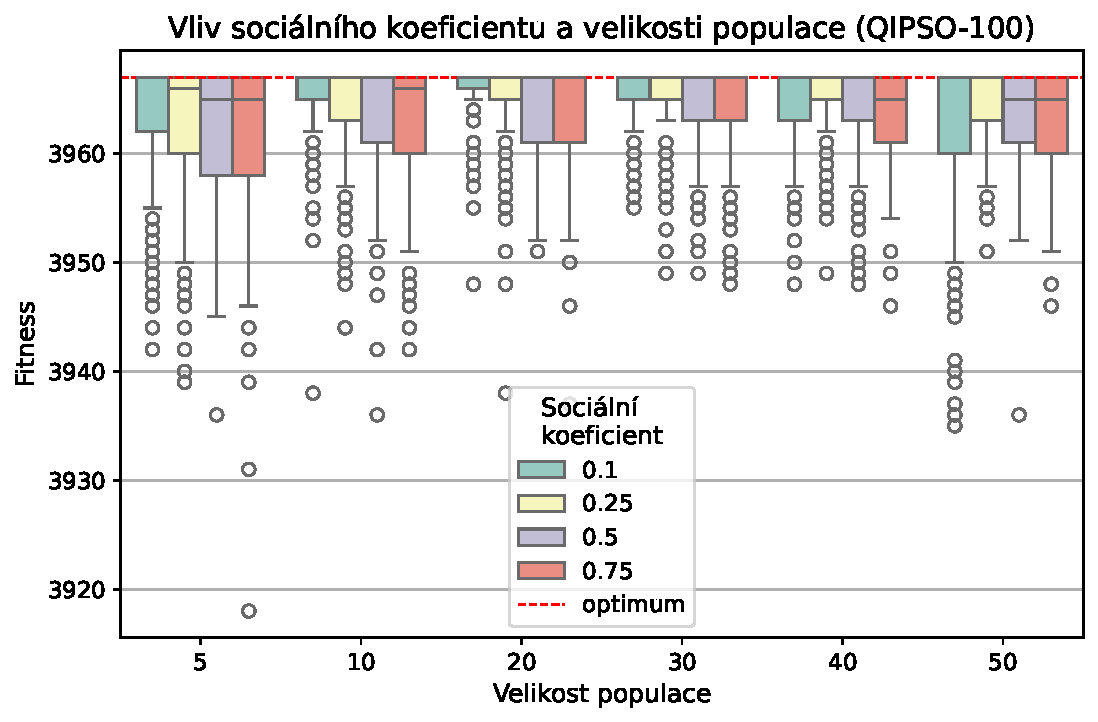
\includegraphics[width=\textwidth]{qipso/boxplot_qipso_100_all_social.pdf}
    \end{subfigure}    
    \caption{Závislost kvality řešení na velikosti populace pro různé hodnoty, po řadě, kognitivního koeficientu a sociálního koeficientu. Data prezentovaná na grafu byla získána algoritmem \emph{QIPSO} na instanci velikosti 100 pomocí 30 nezávislých běhů s 10\,000 evaluacemi na běh pro každou kombinaci testovaných parametrů.}
    \label{fig:qipso-100-all-koeficients}
\end{figure}

\begin{figure}[ht!]
    \centering
    \begin{subfigure}[b]{0.48\textwidth}
        \centering
        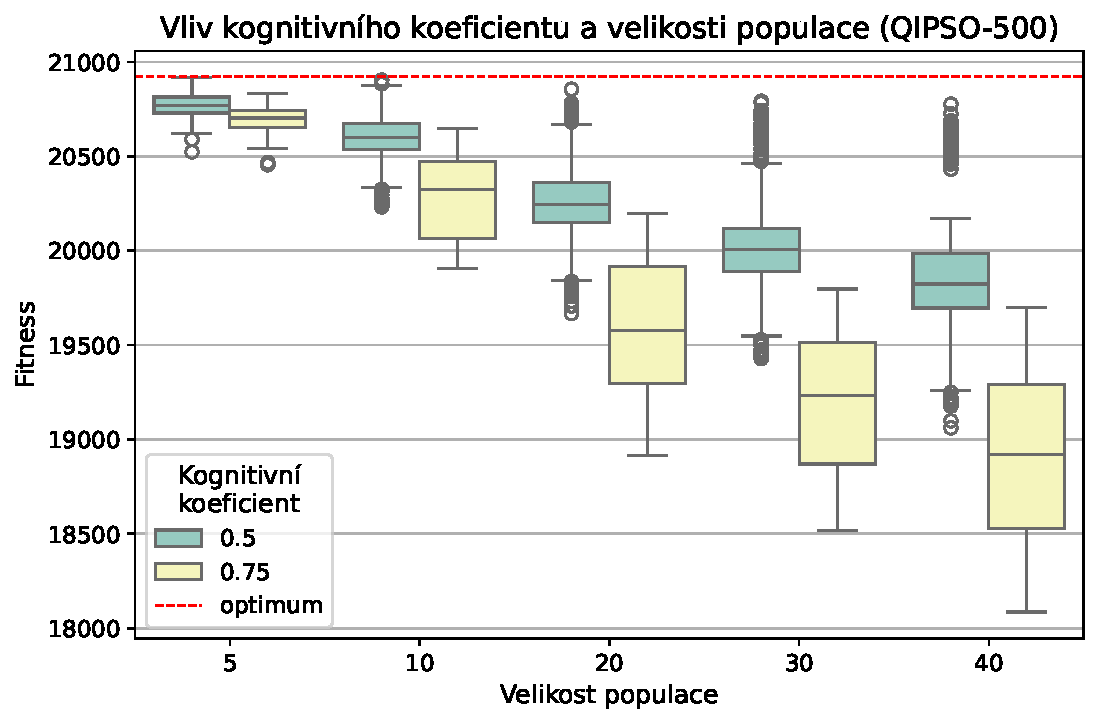
\includegraphics[width=\textwidth]{qipso/boxplot_qipso_500_all_cognitive.pdf}
    \end{subfigure}
    \hfill
    \begin{subfigure}[b]{0.48\textwidth}
        \centering
        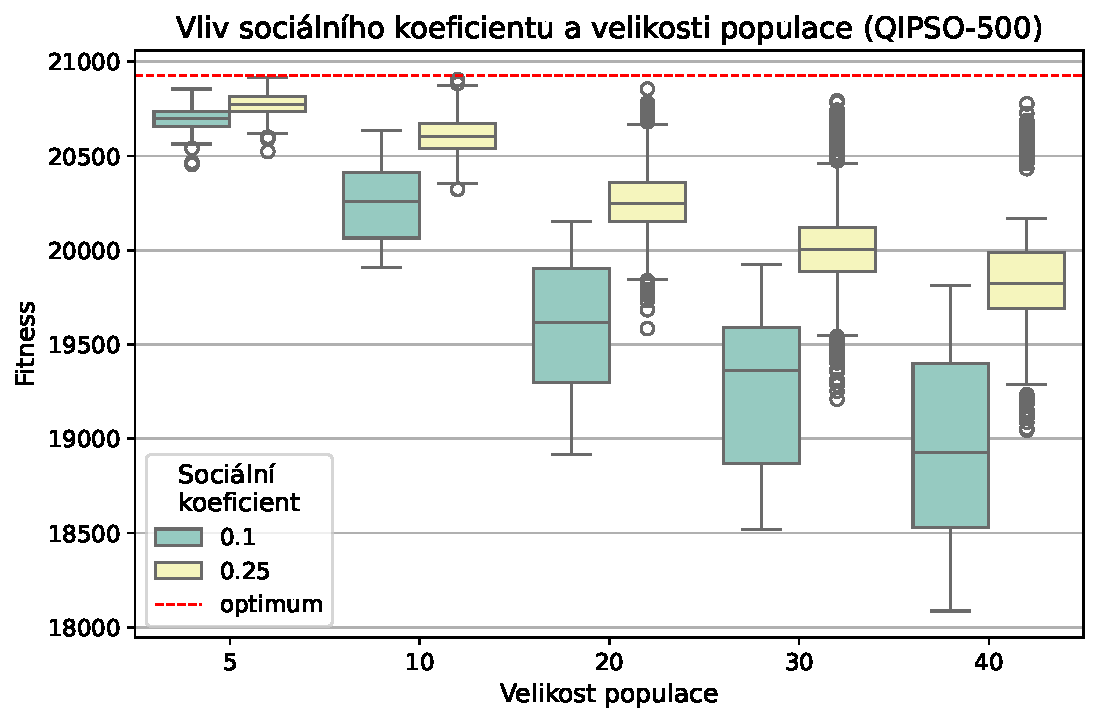
\includegraphics[width=\textwidth]{qipso/boxplot_qipso_500_all_social.pdf}
    \end{subfigure}

    \begin{subfigure}[b]{0.48\textwidth}
        \centering
        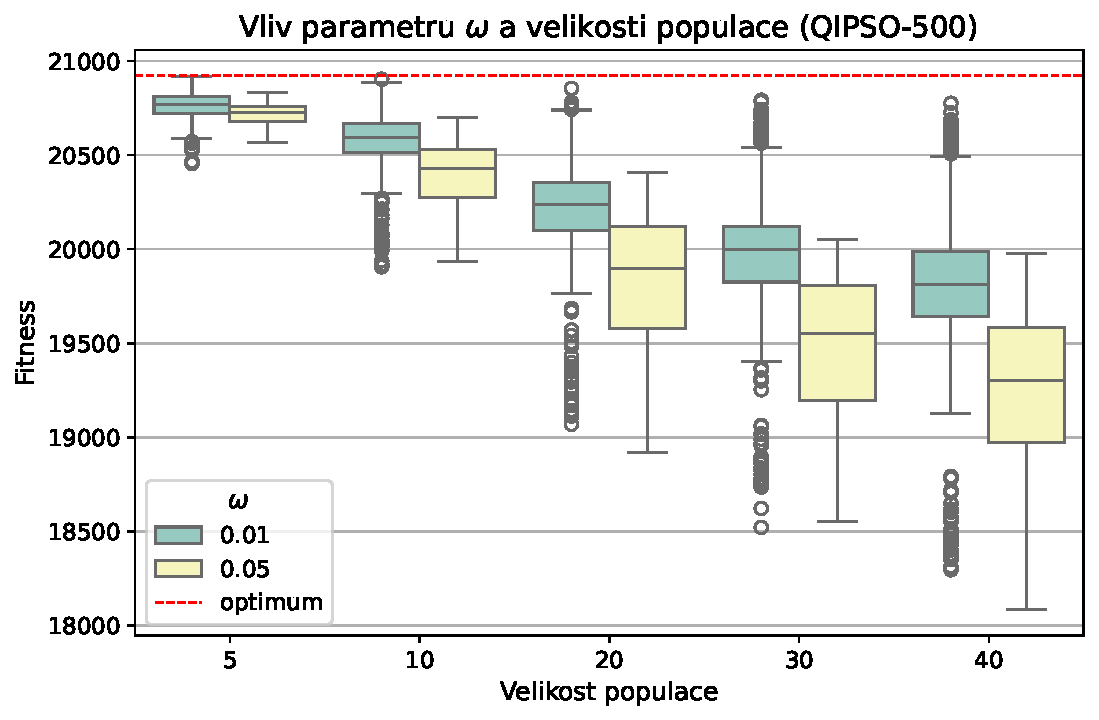
\includegraphics[width=\textwidth]{qipso/boxplot_qipso_500_all_omega.pdf}
    \end{subfigure}
    \caption{Závislost kvality řešení na velikosti populace pro různé hodnoty, po řadě, kognitivního koeficientu, sociálního koeficientu a parametru tření. Data prezentovaná na grafu byla získána algoritmem \emph{QIPSO} na instanci velikosti 500 pomocí 30 nezávislých běhů s 10\,000 evaluacemi na běh pro každou kombinaci testovaných parametrů.}
    \label{fig:qipso-500-koef}
\end{figure}

Graf na obrázku~\ref{fig:qipso-100-all-koeficients} prezentuje závislost kvality řešení na velikosti populace pro různé hodnoty kognitivního a sociálního koeficientu.  
Na základě těchto výsledků budou v dalších experimentech uvažovány hodnoty kognitivního koeficientu 0{,}5 a 0{,}75 a sociálního koeficientu 0{,}1 a 0{,}25, protože tyto kombinace nastavení průměrně poskytovaly nejkvalitnější řešení. 

Vybrané hodnoty kognitivního a sociálního koeficientu spolu s parametry tření byly dále analyzovány na větší instanci o velikosti 500, jak ukazuje obrázek~\ref{fig:qipso-500-koef}.
Z výsledků je patrné, že nejkvalitnějších řešení bylo dosaženo při kognitivním koeficientu 0{,}5, sociálním koeficientu 0{,}25 a parametru tření 0{,}01.
Prezentovaná data na obrázku~\ref{fig:qipso-500-velocity} zobrazující vliv počáteční rychlosti na kvalitu řešení se nejvíce odlišovaly u populace velikosti 50 a 100, přičemž lepších výsledků bylo dosaženo při velikosti 100 a tudíž tato počáteční rychlost společně s výše vybranými hodnotami kognitivního koeficientu, sociálního koeficientu a~parametru tření byly vybrány k další analýze při větších instancích problému. 

\begin{figure}[ht!]
    \centering
    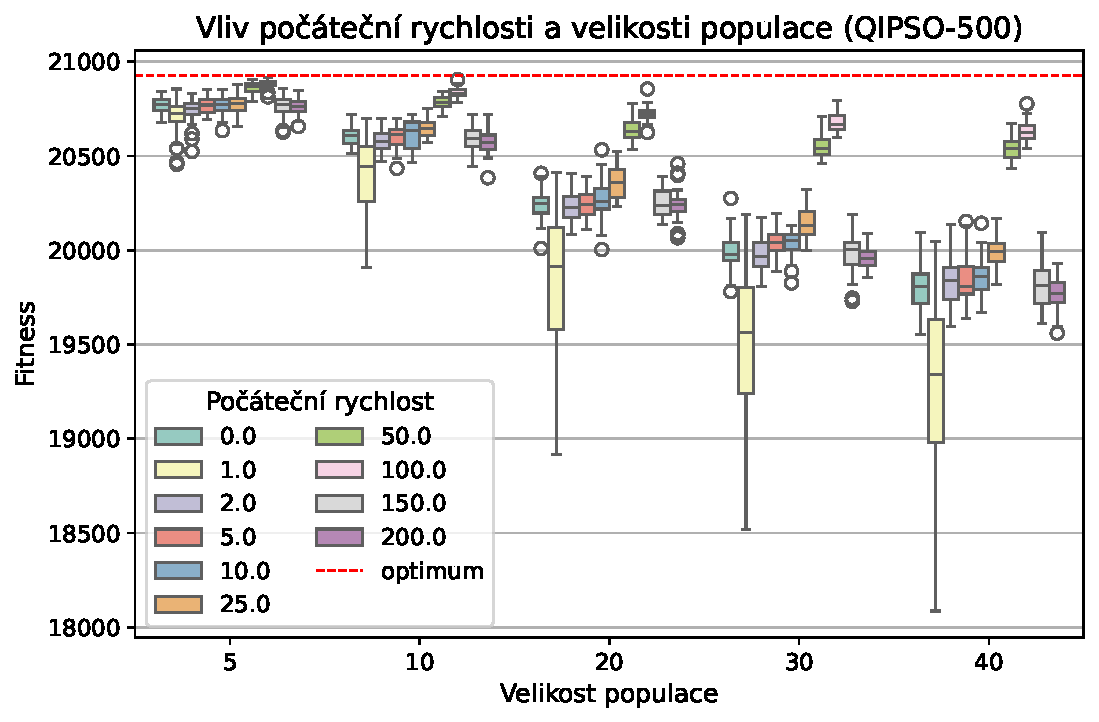
\includegraphics[width=0.98\textwidth]{qipso/boxplot_qipso_500_all_velocity.pdf}
    \caption{Závislost kvality řešení na velikosti populace pro různé hodnoty počáteční rychlosti. Data prezentovaná na grafu byla získána algoritmem \emph{QIPSO} na instanci velikosti 500 pomocí 30 nezávislých běhů s 10\,000 evaluacemi na běh pro každou kombinaci testovaných parametrů.}
    \label{fig:qipso-500-velocity}
\end{figure}

\begin{table}[ht!]
    \centering
    \begin{tabular}{c c c c c c c c c}
        \toprule
        \multirow{2}{*}{\makecell{\textbf{Počáteční}\\\textbf{rychlost}}} & 
        \multirow{2}{*}{\makecell{$\boldsymbol{c_1}$}} & 
        \multirow{2}{*}{\makecell{$\boldsymbol{c_2}$}} &
        \multirow{2}{*}{\makecell{$\boldsymbol{\omega}$}} & 
        \multicolumn{4}{c}{\textbf{Instance}} \\
        \cmidrule(lr){5-8}
        & & & & \textbf{1\,000}    & \textbf{2\,000}     & \textbf{5\,000} & \textbf{10\,000}\\
        \midrule
        100 & 0,5 & 0,25 & 0,01  & 54\,503 & 110\,592 & 275\,805 & 557\,120 \\
        \midrule
        \multicolumn{4}{c}{Optimum} & 54\,503 & 110\,625 & 276\,457 & 563\,647  \\
        \bottomrule
    \end{tabular}
    \caption{Nejlepší dosažené fitness hodnoty algoritmem \emph{QIPSO} pro prezentované nastavení při velkých instancích problému při populaci čítající 5 jedinců.}
    \label{tab:qipso-high-max-values}
\end{table}

\begin{figure}[ht!]
    \centering
    \begin{subfigure}[b]{0.24\textwidth}
      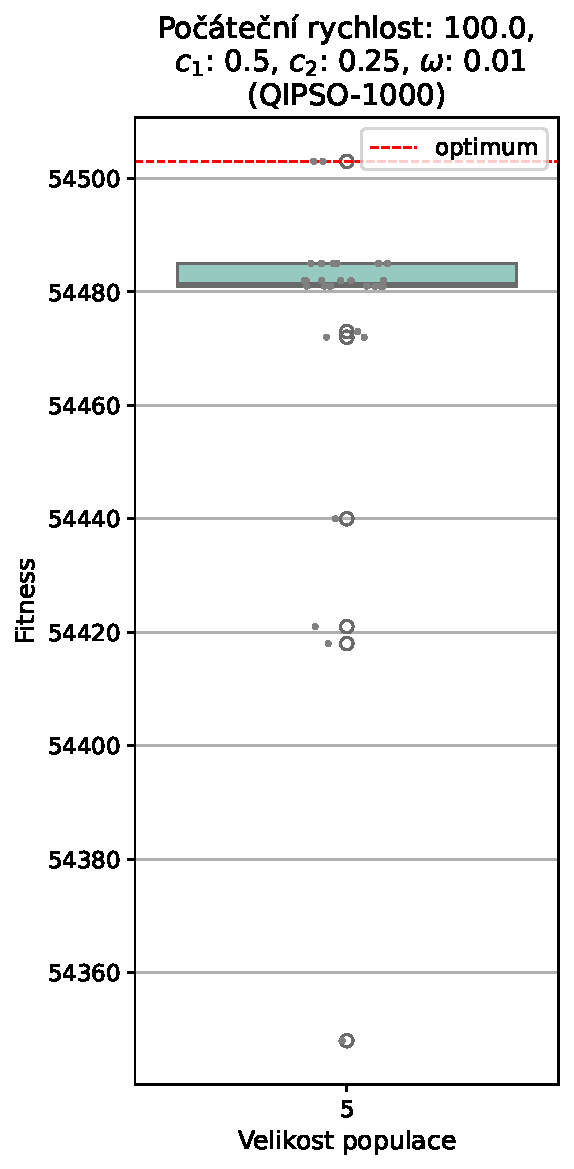
\includegraphics[width=\linewidth]{qipso/boxplot_qipso_1000_large_100.0.pdf}
    \end{subfigure}
    \hfill
    \begin{subfigure}[b]{0.24\textwidth}
        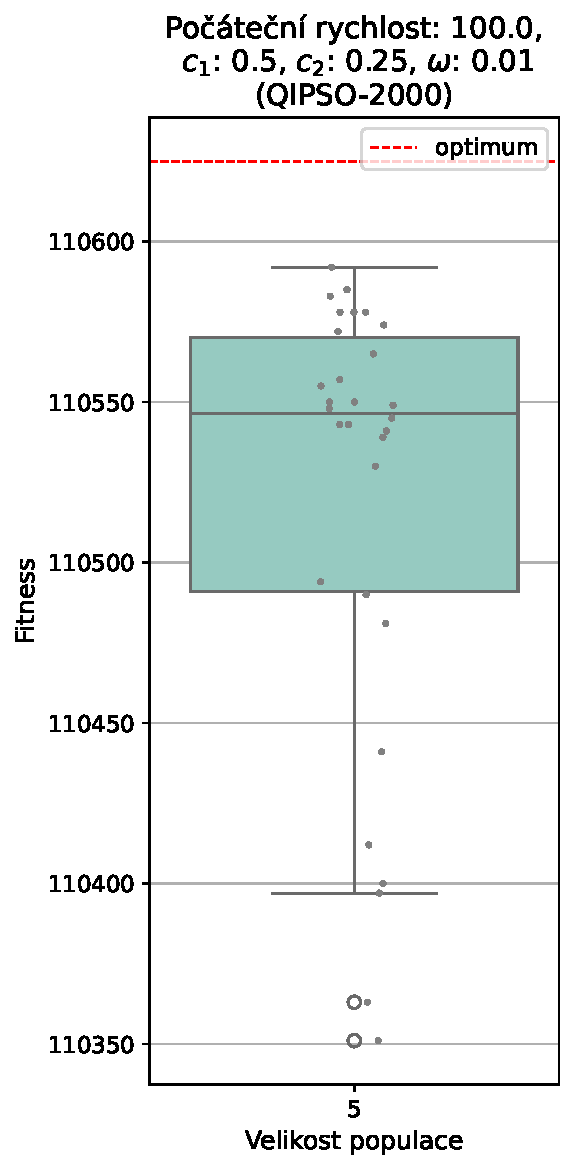
\includegraphics[width=\linewidth]{qipso/boxplot_qipso_2000_large_100.0.pdf}
    \end{subfigure}
    \hfill
    \begin{subfigure}[b]{0.24\textwidth}
        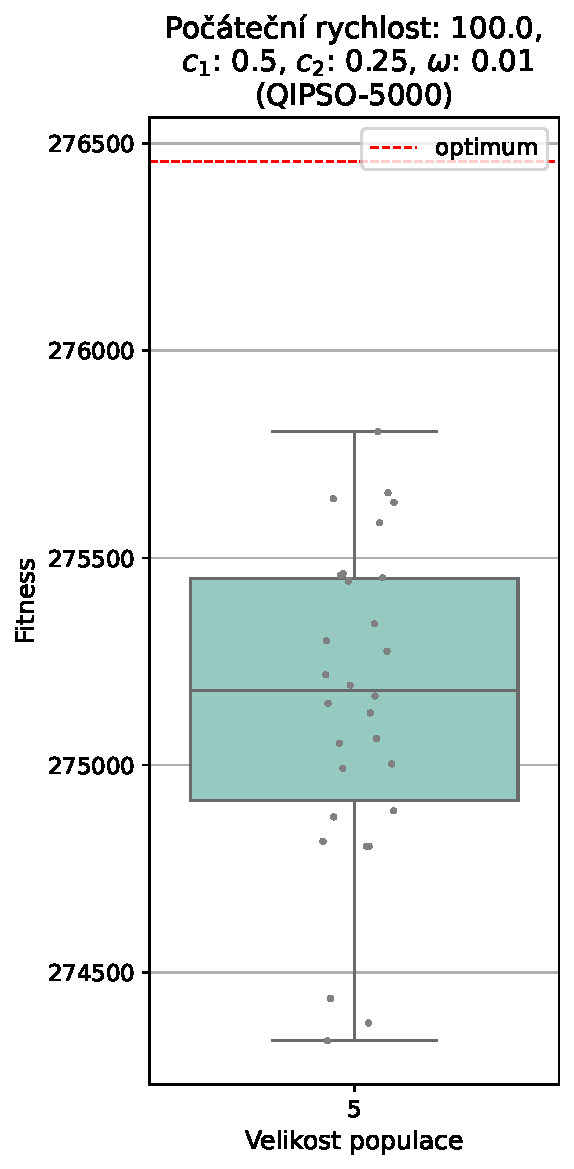
\includegraphics[width=\linewidth]{qipso/boxplot_qipso_5000_large_100.0.pdf}
    \end{subfigure}
    \hfill
    \begin{subfigure}[b]{0.24\textwidth}
        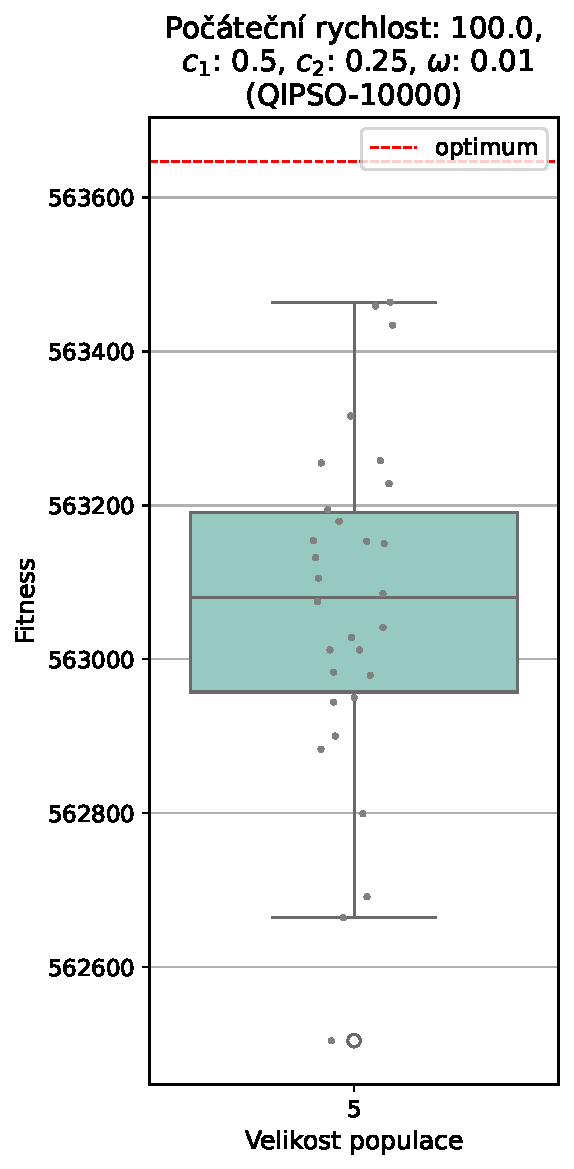
\includegraphics[width=\linewidth]{qipso/boxplot_qipso_10000_large_100.0.pdf}
    \end{subfigure}
    \caption{Porovnání kvality nalezených řešení při hodnotě počáteční rychlosti 100, kognitivního koeficientu $0{,}5$, sociálního koeficientu $0{,}25$, parametru tření $0{,}01$ a pětičlenné populaci při velkých instancích problému. Data prezentovaná na grafu byla získána algoritmem \emph{QIPSO} na instancích, po řadě, velikosti 1\,000, 2\,000, 5\,000 a 10\,000 pomocí 30 nezávislých běhů s 10\,000 evaluacemi na běh.}
    \label{fig:qipso-large}
\end{figure}

Na obrázku~\ref{fig:qipso-large} jsou uvedeny výsledky experimentů provedených na velkých instancích problému s konfigurací algoritmu nastavenou na počáteční rychlost 100, kognitivní koeficient 0{,}5, sociální koeficient 0{,}25, parametr tření 0{,}01 a pětičlennou populaci.
Z grafů a z tabulky~\ref{tab:qipso-high-max-values} nejvyšších dosažených hodnot fitness je patrné, že při velikosti instance 1\,000 algoritmus dosáhl optimálního řešení, zatímco při velikostech instancí 2\,000 a 5\,000 se výsledná řešení pohybovala velmi blízko optimu. 

\newpage
Konvergenční křivky zobrazené na obrázku~\ref{fig:qipso-convergence} ukazují, že v počátečních generacích algoritmu dochází k dočasnému poklesu kvality řešení, který je následně překonán a kvalita nalezených řešení opět vzrůstá.  
Toto chování je způsobeno vysokou počáteční rychlostí částic, kdy dochází k výrazné úpravě pravděpodobnostních koeficientů kvantových chromozomů prostřednictvím kvantového rotačního hradla.

Vlivem vysoké počáteční rychlosti dochází v prvních generacích k rychlému nalezení řešení s relativně vysokou kvalitou. 
V této fázi však převládá explorace, která vede k výrazným změnám v hodnotách pravděpodobnostních koeficientů a k dočasnému opouštění kvalitních oblastí prostoru řešení, což způsobuje dočasný pokles kvality. Následně, jak se rychlost stabilizuje, přechází algoritmus do fáze exploatace, kdy se populace soustředí na vylepšování nalezených kvalitních oblastí a kvalita řešení opět roste.

\begin{figure}[ht!]
    \centering
    \begin{subfigure}[b]{0.48\textwidth}
      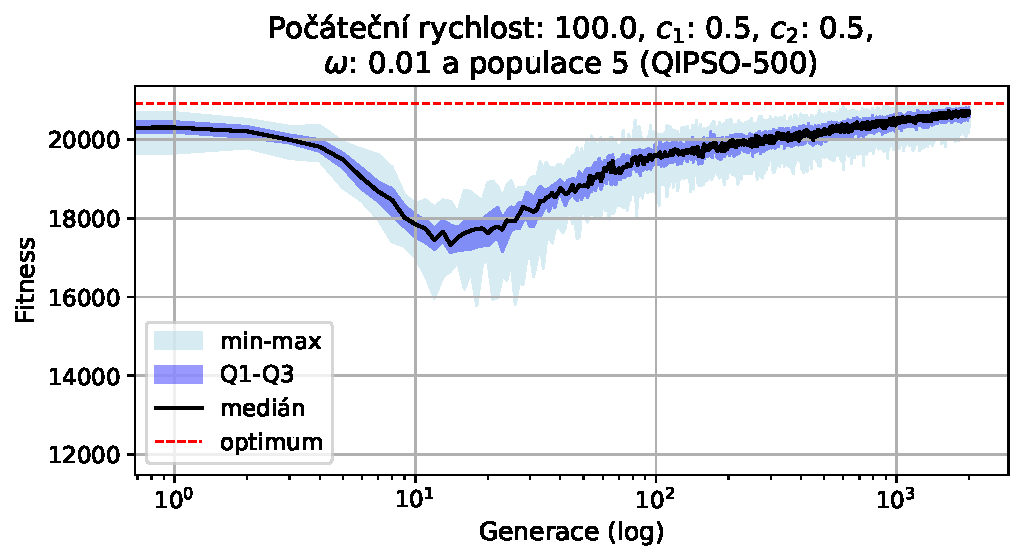
\includegraphics[width=\linewidth]{qipso/qipso_convergence_500_velocity_100.0_population_5.pdf}
    \end{subfigure}
    \hfill
    \begin{subfigure}[b]{0.48\textwidth}
        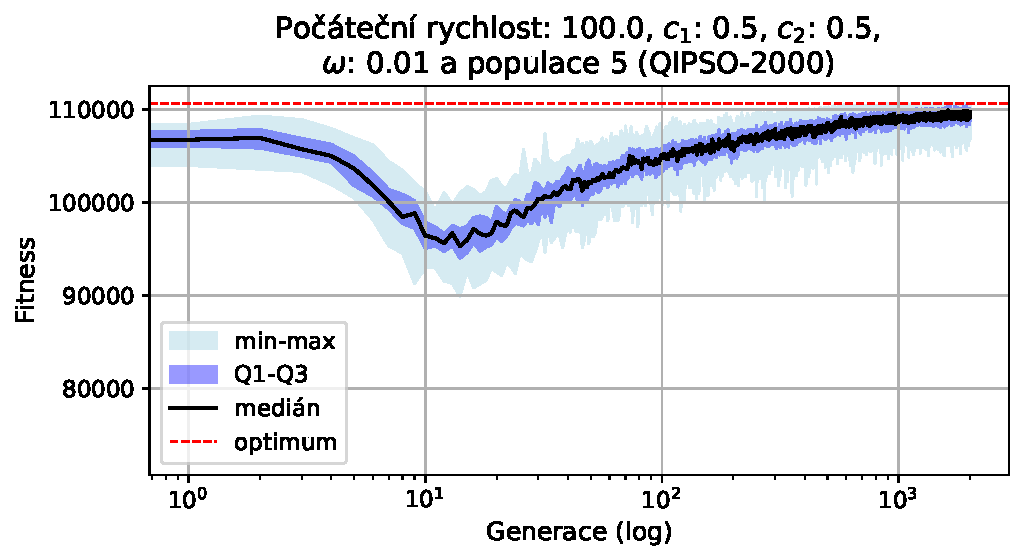
\includegraphics[width=\linewidth]{qipso/qipso_convergence_2000_c1_0.5_c2_0.25_omega_0.01_velocity_100.0_population_5.pdf}
    \end{subfigure}
    \caption{Konvergenční křivky algoritmu, jehož parametr počáteční rychlosti byl nastaven na 100, kognitivního koeficientu na $0{,}5$, sociálního koeficientu na $0{,}25$, parametru tření na $0{,}01$ při pětičlenné populaci. Data prezentovaná na grafu byla získána algoritmem \emph{QIPSO} na instancích, po řadě, velikosti 500 a 2\,000 pomocí 30 nezávislých běhů s 10\,000 evaluacemi na běh.}
    \label{fig:qipso-convergence}
\end{figure}

\section{Srovnání algoritmů a diskuze}
V této sekci jsou nejprve navzájem porovnány kvantově inspirované evoluční algoritmy \emph{QIGA}, \emph{QISA}, \emph{QSE} a \emph{QIPSO}, jež byly popsány, po řadě, v sekcích~\ref{sec:qiga},~\ref{sec:qisa},~\ref{sec:qse} a~\ref{sec:qipso} a~jejichž doladěné parametry byly představeny, po řadě, v sekcích~\ref{sec:exp-qiga},~\ref{sec:exp-qisa},~\ref{sec:exp-qse} a~\ref{sec:exp-qipso}, přičemž přehled těchto parametrů a jejich hodnot pro jednotlivé algoritmy je uveden v tabulce~\ref{tab:best-configs}. 
Tyto konfigurace byly následně využity ve všech srovnávacích experimentech. 
Po tomto vzájemném porovnání budou kvantově inspirované algoritmy dále srovnány s vybranými běžně používanými optimalizačními metodami. 

\begin{table}[ht]
    \centering
    \begin{tabularx}{\textwidth}{c X c}
        \toprule
        \textbf{Algoritmus} & \textbf{Konfigurace parametrů} & \textbf{Velikost populace} \\
        \midrule
        QIGA   & $\Delta\theta = 0{,}002$ & 1 \\[1ex]
        QISA   & rekurzivně-logaritmický chladicí plán a sigmoidní zahřívací funkce & 1 \\[1ex]
        QSE    & počáteční rychlost = 1 & 5 \\[1ex]
        QIPSO  & počáteční rychlost = 100, $c_1 = 0{,}5$, $c_2 = 0{,}25$, $\omega = 0{,}01$ & 5 \\
        \bottomrule
    \end{tabularx}
    \caption{Nejlepší nalezené hodnoty parametrů pro jednotlivé algoritmy.}
    \label{tab:best-configs}
\end{table}

Na obrázku~\ref{fig:best-10k} jsou znázorněny výsledky experimentů porovnávajících jednotlivé kvantově inspirované evoluční algoritmy na větších instancích problému, přičemž jejich konfigurace odpovídá parametrům uvedených v tabulce~\ref{tab:best-configs}. 

Z výsledků uvedených v tabulce~\ref{tab:qiea-comparsion} a na obrázku~\ref{fig:best-10k} je patrné, že žádný z kvantově inspirovaných evolučních algoritmů, co se týče kvality vyvinutých výsledků velmi nezaostává. 
U instance o velikosti 1\,000 položek se všechny algoritmy blíží optimální hodnotě, přičemž algoritmu \emph{QIPSO} se jako jedinému podařilo nalézt řešení, jehož fitness odpovídá přímo optimální hodnotě. 

S rostoucími velikostmi instancí se mezi algoritmy začínají výrazněji projevovat rozdíly v kvalitě nalezených řešení. 
Algoritmus \emph{QIPSO} dosahuje nejlepších výsledků ve všech testovaných instancích a nejvíce se přibližuje známému optimu i při instancích o velikosti 5\,000 a~10\,000. 
Naopak algoritmy \emph{QIGA} a \emph{QSE} vykazují u větších instancí výraznější odchylky od optimální hodnoty, kdy se algoritmus \emph{QSE} vzdaluje optimu již od velikosti instance 2\,000, zatímco algoritmus \emph{QIGA} se začíná mírně vzdalovat až od velikosti instance 5\,000. 

\begin{table}[H]
    \centering
    \begin{tabular}{c c c c c}
        \toprule
        \multirow{2}{*}{\makecell{\textbf{Algoritmus}}} & 
        \multicolumn{4}{c}{\textbf{Instance}} \\
        \cmidrule(lr){2-5}
         & \textbf{1\,000}    & \textbf{2\,000}     & \textbf{5\,000} & \textbf{10\,000}\\
        \midrule
        QIGA  & 54\,485 & 110\,373 & 272\,306 & 530\,066 \\[1ex]
        QISA  & 54\,481 & 110\,287 & 274\,150 & 548\,460 \\[1ex]
        QSE   & 54\,481 & 108\,387 & 267\,827 & 544\,824 \\[1ex]
        QIPSO & 54\,503 & 110\,592 & 275\,805 & 557\,120 \\
        \midrule
        \multicolumn{1}{c}{Optimum} & 54\,503 & 110\,625 & 276\,457 & 563\,647  \\
        \bottomrule
    \end{tabular}
    \caption{Nejlepší dosažené fitness hodnoty jednotlivými kvantově inspirovanými evolučními algoritmy při konfiguraci jejich parametrů dle tabulky~\ref{tab:best-configs} pro 10\,000 evaluací.}
    \label{tab:qiea-comparsion}
\end{table}

\begin{figure}[ht!]
    \centering
    \begin{subfigure}[b]{0.48\textwidth}
      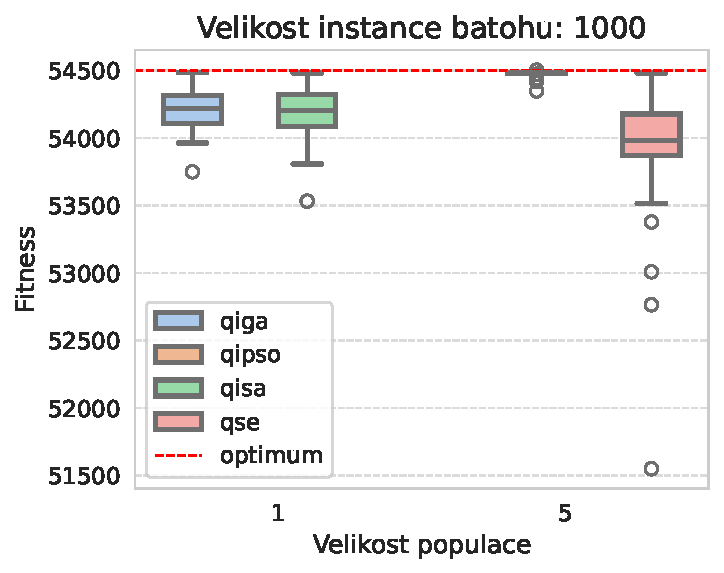
\includegraphics[width=\linewidth]{best/best_all_qiea_1000.pdf}
    \end{subfigure}
    \hfill
    \begin{subfigure}[b]{0.48\textwidth}
        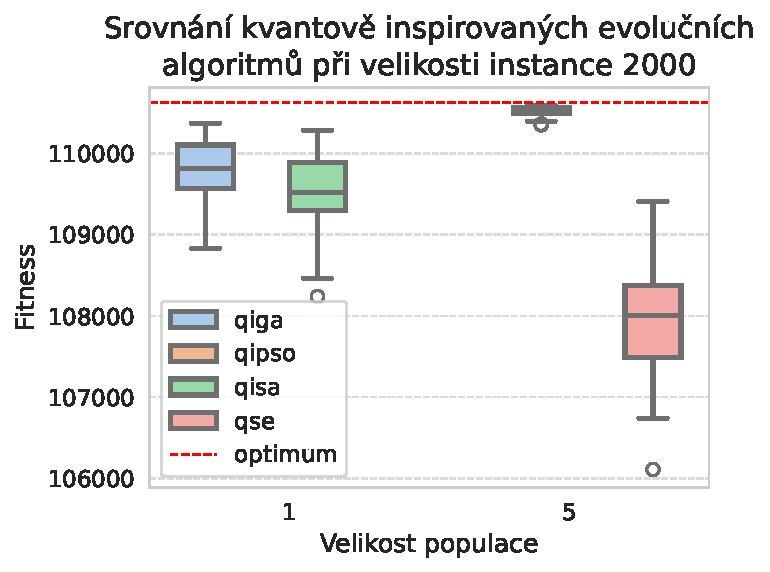
\includegraphics[width=\linewidth]{best/best_all_qiea_2000.pdf}
    \end{subfigure}

    \begin{subfigure}[b]{0.48\textwidth}
      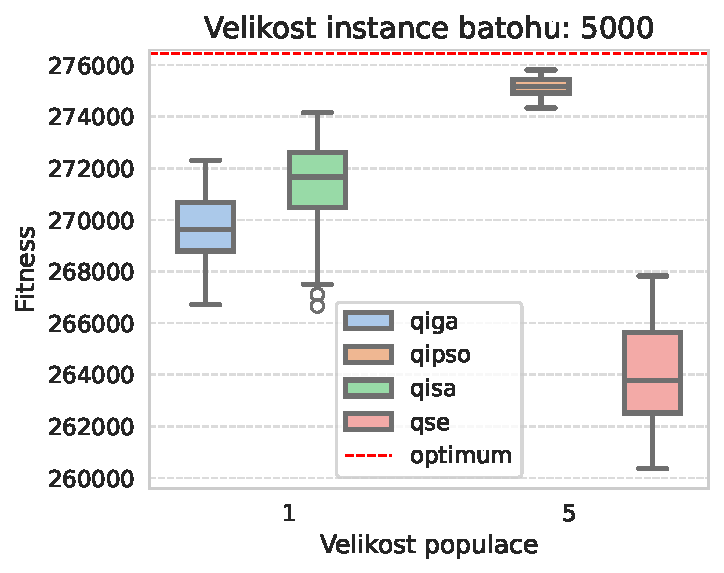
\includegraphics[width=\linewidth]{best/best_all_qiea_5000.pdf}
    \end{subfigure}
    \hfill
    \begin{subfigure}[b]{0.48\textwidth}
        \includegraphics[width=\linewidth]{best/best_all_qiea_10000.pdf}
    \end{subfigure}
    \caption{Data prezentovaná na grafu byla získána, po řadě, algoritmy \emph{QIGA}, \emph{QISA}, \emph{QSE} a \emph{QIPSO} na instancích, po řadě, velikosti 1\,000, 2\,000, 5\,000 a 10\,000 pomocí 30 nezávislých běhů s 10\,000 evaluacemi na běh.}
    \label{fig:best-10k}
\end{figure}

Na obrázku~\ref{fig:best-100k} a v tabulce~\ref{tab:max-fitness-10000} jsou prezentovány získané fitness hodnoty pomocí jednotlivých kvantově inspirovaných evolučních algoritmů na instanci o velikosti 10\,000 položek, přičemž každý běh měl k~dispozici 100\,000 evaluací.
Tento experiment byl proveden za účelem ověření, jakého výkonu jsou algoritmy schopny dosáhnout, pokud jim bude na rozsáhlých instancích poskytnut větší výpočetní prostor.

Ve srovnání s předchozími experimenty, kde bylo použito pouze 10\,000 evaluací, se ukazuje, že prodloužený běh umožňuje většině algoritmů lépe prozkoumat prostor řešení a~nalézt kvalitnější výsledky. 
Výjimkou je algoritmus \emph{QSE}, který na rozdíl od ostatních algoritmů zaznamenal pouze minimální zlepšení ve kvalitě nalezených řešení. 
Výraznějšího zlepšení, a~to jak z hlediska kvality generovaných řešení, tak jejich stability, dosáhl algoritmus \emph{QISA}, avšak nejlepšího výsledku opět dosáhl algoritmus \emph{QIPSO}, jenž se výrazně přiblížil optimální hodnotě. 

\begin{figure}[ht!]
    \centering
    \includegraphics[width=0.6\textwidth]{best_all_qiea_10000.pdf}
    \caption{Data prezentovaná na grafu byla získána, po řadě, algoritmy \emph{QIGA}, \emph{QISA}, \emph{QSE} a \emph{QIPSO} na instanci velikosti a 10\,000 pomocí 30 nezávislých běhů s 100\,000 evaluacemi na běh.}
    \label{fig:best-100k}
\end{figure}

\begin{table}[ht]
    \centering
    \begin{tabular}{l c}
        \toprule
        \textbf{Algoritmus} & \textbf{Maximální fitness} \\
        \midrule
        QIGA    & 552\,513 \\[1ex]
        QISA    & 562\,368 \\[1ex]
        QSE     & 545\,171 \\[1ex]
        QIPSO   & 563\,464 \\
        \midrule
        Optimum & 563\,647 \\
        \bottomrule
    \end{tabular}
    \caption{Nejlepší dosažené fitness hodnoty jednotlivými kvantově inspirovanými evolučními algoritmy při konfiguraci jejich parametrů dle tabulky~\ref{tab:best-configs} pro 100\,000 evaluací.}
    \label{tab:max-fitness-10000}
\end{table}

Výsledky kvantově inspirovaných evolučních algoritmů byly porovnány s běžnými optimalizačními metodami, které byly představeny ve studii~\cite{compare}.  
Tato studie byla zvolena mimo jiné proto, že využívá stejné datové sady, jaké byly použity v této práci, vizte tabulka~\ref{tab:experiments-design}, což umožňuje přímé porovnání dosažených výsledků.

Ve zmíněné studii byly experimentálně testovány následující algoritmy:
\begin{itemize}
    \item simulované žíhání \emph{(Simulated Annealing\,--\,SA)}~\cite{sa},
    \item genetický algoritmus \emph{(Genetic Algorithm\,--\,GA)}~\cite{ga-app},
    \item hladový algoritmus \emph{(Greedy Search Algorithm\,--GSA)}~\cite{GSA},
    \item dynamické programování \emph{(Dynamic Programming\,--\,DP)}~\cite{DP} a 
    \item metoda větví a mezí \emph{(Branch and Bound\,--\,BB)}~\cite{BB}.
\end{itemize}
Výsledky těchto metod jsou společně s výsledky kvantově inspirovaných evolučních algoritmů uvedeny v tabulce~\ref{tab:alg-comparison}.

\begin{table}[ht]
    \centering
    \begin{tabular}{c c c c c}
        \toprule
        \multirow{2}{*}{\textbf{Algoritmus}} &
        \multicolumn{4}{c}{\textbf{Instance}} \\
        \cmidrule(lr){2-5}
              & 1\,000  & 2\,000   & 5\,000   & 10\,000 \\
        \midrule
        SA    & 36\,179 &  65\,793 & 150\,731 & 563\,647 \\[1ex]
        GA    &     130 & 102\,340 & 102\,340 & 562\,556 \\[1ex]
        GSA   & 14\,927 &  25\,579 &  49\,306 & 292\,225 \\[1ex]
        DP    & 54\,503 & 110\,625 & 276\,457 & 106\,464 \\[1ex]
        BB    & 53\,397 & 109\,679 & 275\,720 &      130 \\[1ex]
        QIGA  & 54\,485 & 110\,373 & 272\,306 & 552\,513 \\[1ex]
        QISA  & 54\,481 & 110\,287 & 274\,150 & 562\,368 \\[1ex]
        QSE   & 54\,481 & 108\,387 & 267\,827 & 545\,171 \\[1ex]
        QIPSO & 54\,503 & 110\,592 & 275\,805 & 563\,464 \\
        \midrule
        Optimum & 54\,503 & 110\,625 & 276\,457 & 563\,647 \\
        \bottomrule
    \end{tabular}
    \caption{Nejlepší dosažené fitness hodnoty jednotlivými algoritmy.}
    \label{tab:alg-comparison}
\end{table}

Tabulka~\ref{tab:alg-comparison} shrnuje nejlepší dosažené hodnoty fitness jednotlivých algoritmů na instancích různých velikostí.
Z výsledků je patrné, že exaktní algoritmy~\cite{compare}, jako jsou \emph{DP} a~\emph{BB}, poskytují optimální nebo téměř optimální řešení pro instance velikosti 1\,000, 2\,000 a~5\,000, ale u instance o velikosti 10\,000 jejich výkonnost znatelně klesá. 
Heuristiky \emph{SA} a~\emph{GA} obecně dosahují nižší kvality řešení, avšak u instance 10\,000 poskytly výsledky blízké optimální hodnotě a v případě algoritmu \emph{SA} se dokonce podařilo nalézt řešení, jehož kvalita odpovídá známému optimu.

Kvantově inspirované evoluční algoritmy dosahují stabilně vysokých hodnot fitness napříč všemi testovanými instancemi. 
Nejlepší výkonnost opakovaně prokazuje navržený algoritmus \emph{QIPSO}, který se výrazně přibližuje známému optimu i u největších instancí.
Také algoritmy \emph{QISA} a \emph{QIGA} poskytují konkurenceschopné výsledky, přičemž \emph{QSE} mírně zaostává, zejména u rozsáhlejších úloh.
